\documentclass[10pt]{article}

\usepackage{hyperref} 
\usepackage{graphicx} 
\usepackage{fancybox} 
\usepackage{rotating} 
\usepackage{color} 
\usepackage{DIN_A4} 
\usepackage{here}

\ifx\MARaBOU\undefined
\def\MARaBOU{MAR\lower.5ex\hbox{a}BO\kern-.5em\lower.5ex\hbox{O}\kern-.1em U}%
\fi

\newcommand{\samefootnote}{$^\alph{footnote}$}
\newcommand{\samempfootnote}{$^\alph{mpfootnote}$}

\definecolor{lightblue}{rgb}{.68,.88,.90}

\newcommand{\blue}[1]{\colorbox{lightblue}{\texttt{#1}}}

\newenvironment{boxed}
	{\begin{Sbox}\begin{minipage}[t]}
	{\end{minipage}\end{Sbox}\fbox{\TheSbox}}
	
\newenvironment{yellowboxed}
	{\begin{Sbox}\begin{minipage}[t]}
	{\end{minipage}\end{Sbox}\colorbox{yellow}{\TheSbox}}
	
\newenvironment{blueboxed}
	{\begin{Sbox}\begin{minipage}[t]}
	{\end{minipage}\end{Sbox}\colorbox{lightblue}{\TheSbox}}
	

\setlength{\parindent}{0pt}

\begin{document}
\begin{titlepage}
\title{MED Data Structure}
\author{R. Lutter}
\maketitle
\vfill
\begin{abstract}
This document describes the structure of experimental data taken in MINIBALL experiments
using the \MARaBOU{} data acquisition system.
\textbf{MED} is an abbreviation for
"\textbf{M}BS \textbf{E}vent \textbf{D}ata" as this format
is based on regular MBS data structures \cite{GoosyBufferStructure}.\\
A detailed description of MBS data structures used as well as \MARaBOU{} extensions to these structures will be given.
\end{abstract}
\vfill\vfill
\end{titlepage}
\newpage
\tableofcontents
\newpage
\section{MED file format}
A \texttt{\textbf{.med}} file contains a stream of MBS events of standard type [10,1]
(known as "\texttt{VME Event}" inside MBS).
In contrast to the MBS file format (\texttt{\textbf{.lmd}} format) no buffering is used during output:
data are streamed out event by event by the generating program.
As a consequence there is no event spanning across buffer boundaries making things easier for the reader.
Note that there is neither a file header nor any buffer header, too.
Each event contains a sequence of subevents all based on MBS subevent [10,1] (so-called "\texttt{CAMAC Subevent}").
There are several extensions to this subevent type to cover different hardware and software requirements within \MARaBOU{}.\\
Fig.\,\ref{MedFileFormat} shows the overall MED data structure,
table\,\ref{MarabouSubevents} gives a list of subevent types used by \MARaBOU{} applications \cite{MarabouHomePage}.
\begin{figure}[H]
\centerline{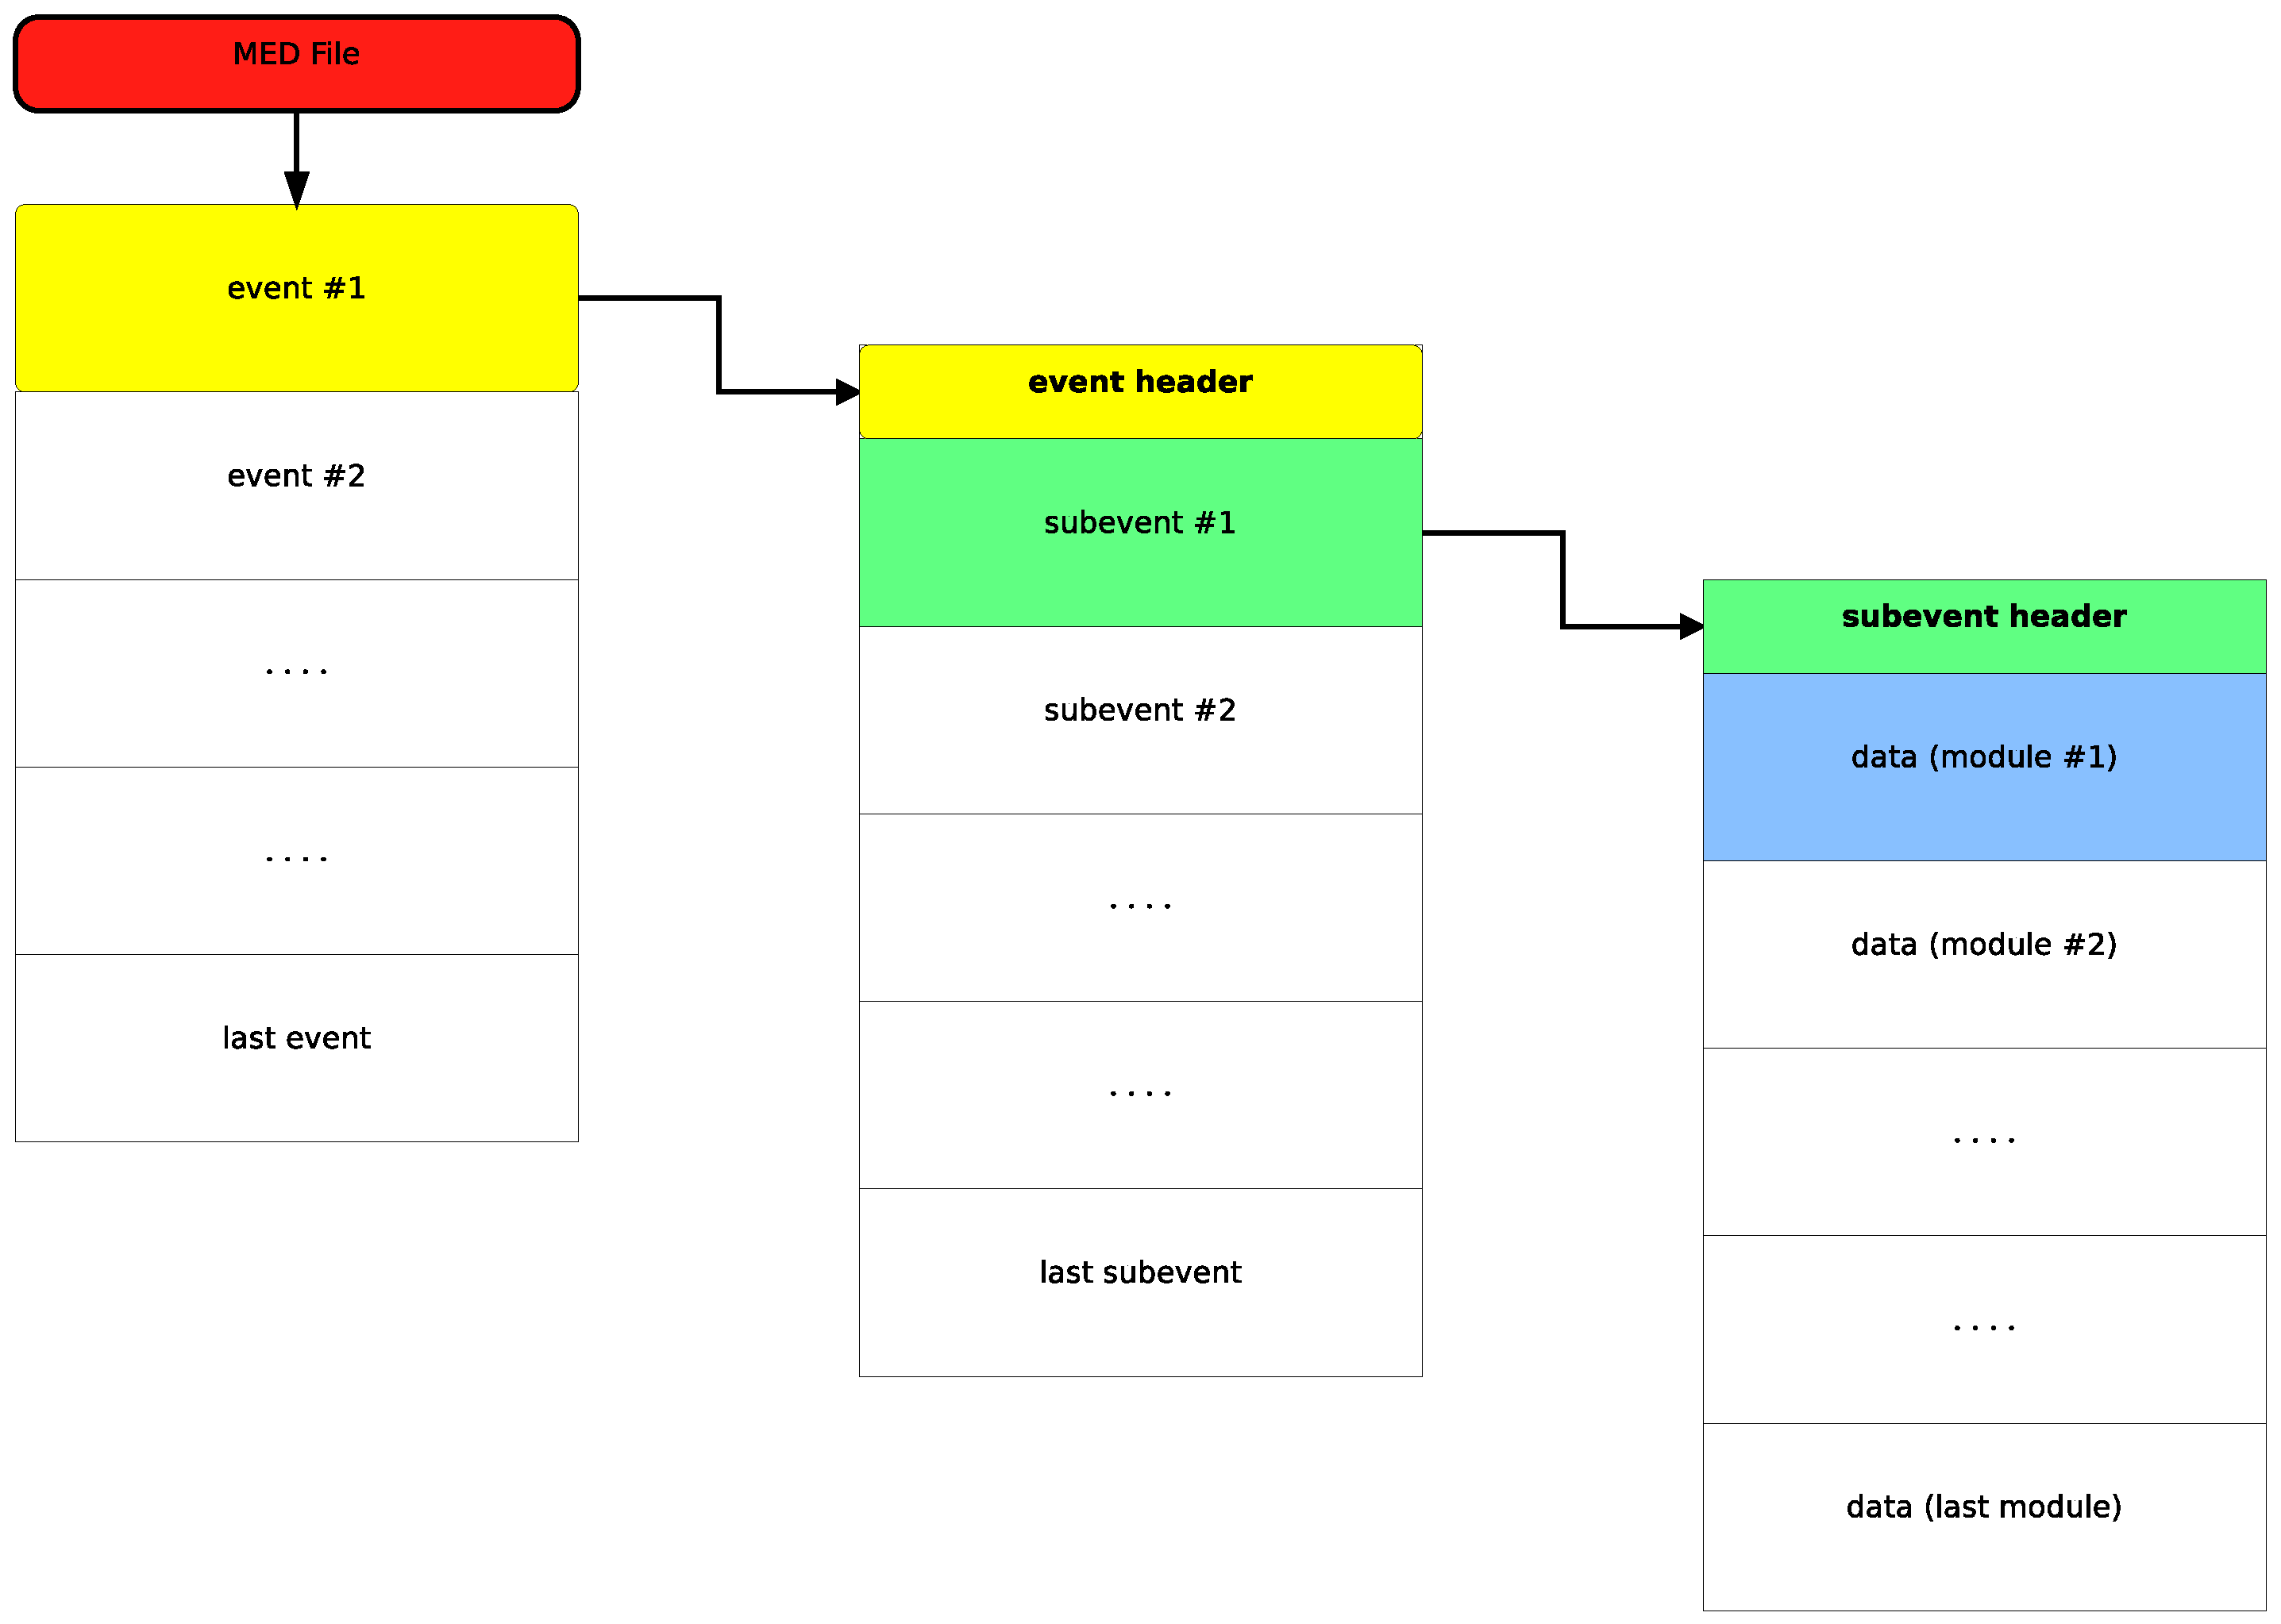
\includegraphics[width=\linewidth]{MedFileStructure}}
\caption{Overall structure of MED data}
\label{MedFileFormat}
\end{figure} 
\begin{sidewaystable}
\begin{center}
\begin{tabular}{|l|l|l|l|l|}
\hline
\verb+[type,subtype]+ & class name & format & mps\,\footnote{modules per subevent} & comment \\
\hline\hline
\verb+[10,1]+ & \verb+TMrbSubevent_10_1+ & zero-compressed, data preceeded by channel number & 1 only & universal MBS subevent \\
\hline
\verb+[10,11]+ & \verb+TMrbSubevent_10_11+ & data w/o channel numbers, zero-padded & 1 only / any
\footnote{As there is no module id in this format the sequence of modules has to be
known to the reader. To avoid ambiguities it is recommended to store 1 module per subevent only.} & universal \MARaBOU{} subevent \\
\verb+[10,12]+ & \verb+TMrbSubevent_10_12+ & same as \verb+[10,1]+, including module headers & any & \\
\hline
\verb+[10,21]+ & \verb+TMrbSubevent_DGF_1+ & original XIA format & any & for XIA DGF-4C modules \\
\verb+[10,22]+ & \verb+TMrbSubevent_DGF_2+\,\footnote{Note: formats \texttt{2} and \texttt{3} have \textbf{same}
data structure on input but follow different output strategies} &  \dots & any &  \dots \\
\verb+[10,23]+ & \verb+TMrbSubevent_DGF_3+\,\samempfootnote &  \dots & any &  \dots \\
\hline
\verb+[10,31]+ & \verb+TMrbSubevent_Silena_1+ &  zero-compressed Silena format & any &  for Silena 4418V/T modules \\
\verb+[10,32]+ & \verb+TMrbSubevent_Silena_2+\,\samempfootnote &  \dots & any &  \dots \\
\hline
\verb+[10,41]+ & \verb+TMrbSubevent_Caen_1+ & original CAEN format & any & for CAEN V785/V775 modules \\
\verb+[10,42]+ & \verb+TMrbSubevent_Caen_2+\,\samempfootnote &  \dots & any &  \dots \\
\verb+[10,43]+ & \verb+TMrbSubevent_Caen_3+\,\samempfootnote &  \dots & any &  \dots \\
\hline
\verb+[10,51]+ & \verb+TMrbSubevent_Sis_1+ & original SIS format & any & for SIS 3XXX modules \\
\verb+[10,52]+ & \verb+TMrbSubevent_Sis_2+\,\samempfootnote &  \dots & any &  \dots \\
\verb+[10,53]+ & \verb+TMrbSubevent_Sis_3+\,\samempfootnote &  \dots & any &  \dots \\
\hline
\verb+[10,91]+ & \verb+TMrbSubevent_Data_S+ & short (16 bit) data & -- & universal data container \\
\verb+[10,92]+ & \verb+TMrbSubevent_Data_I+ & int (32 bit) data & -- & \dots \\
\verb+[10,93]+ & \verb+TMrbSubevent_Data_F+ & float (32 bit) data & -- & \dots \\
\hline
\verb+[9000,1]+ & & time stamp & -- &  ppc clock, in steps of 100 $\mu$s \\
\verb+[9000,2]+ & & dead time & -- &  contents of dead time scaler \\
\verb+[111,111]+ & & default & -- & default (empty) subevent \\
\hline
\end{tabular} 
\caption{Subevent types used by \MARaBOU{}}
\label{MarabouSubevents}\end{center}
\end{sidewaystable}
\section{Event and subevent formats used by \MARaBOU{}}
Fig.\,\ref{MedStandardHeaders} shows standard MBS event and subevent headers as used in a \MARaBOU{}
environment.
\begin{figure}[H]
\centerline{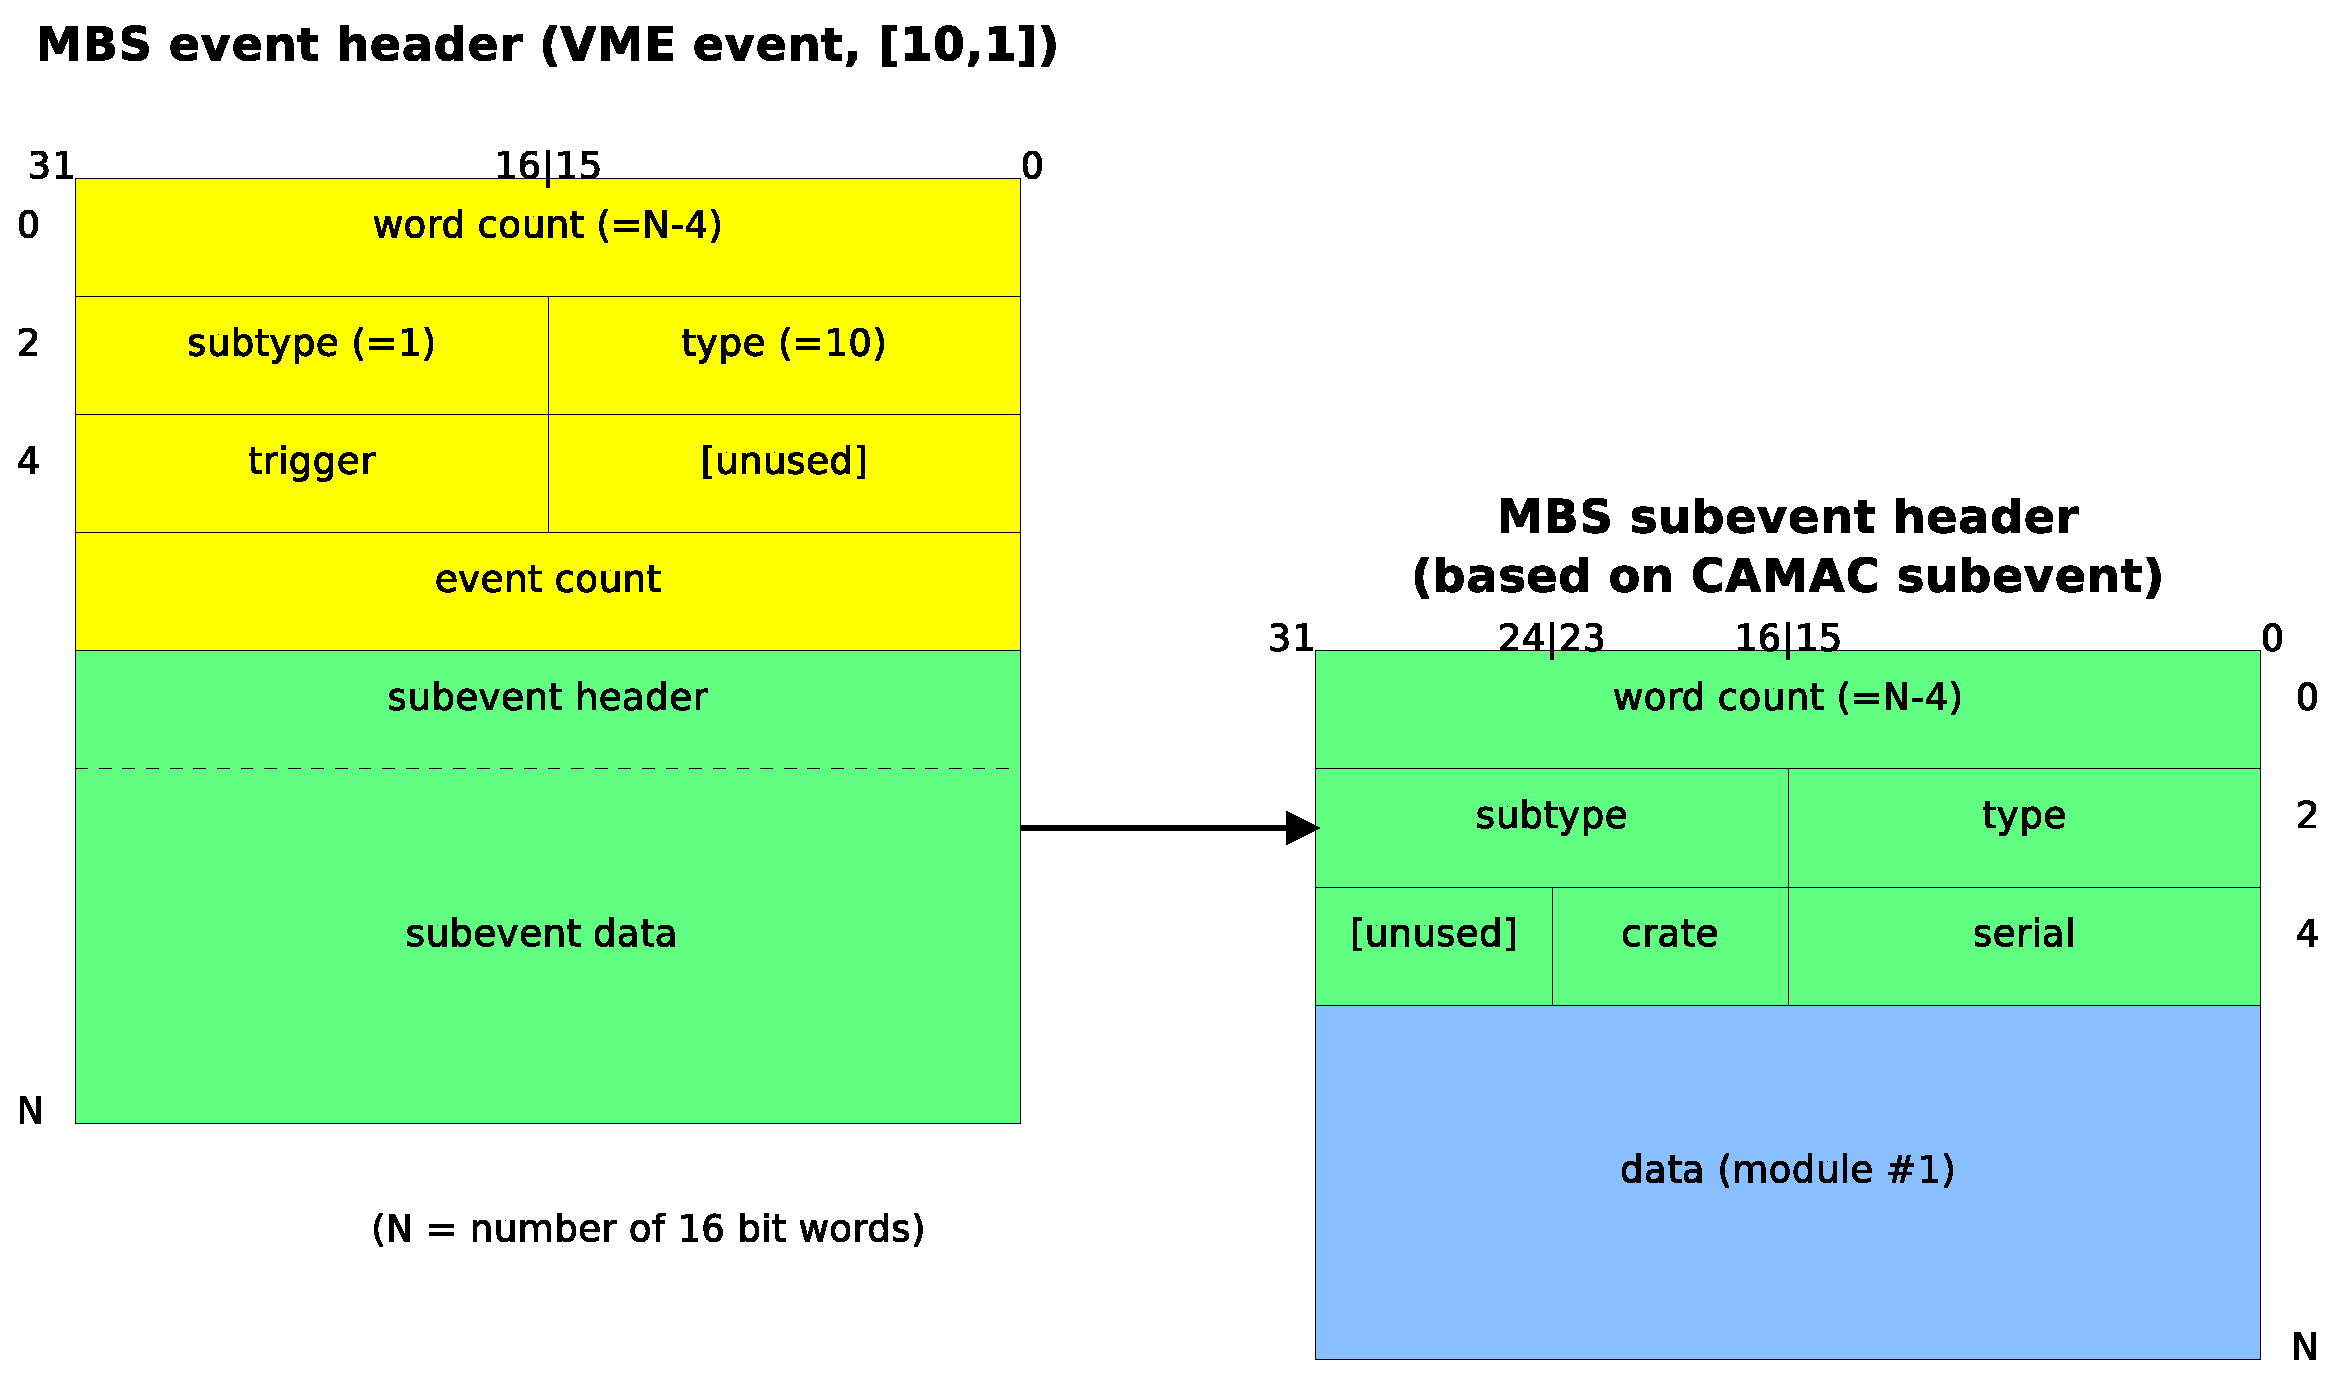
\includegraphics[width=\linewidth]{MedStandardHeaders}}
\caption{Standard MBS headers used in \MARaBOU{}\,\cite{GoosyBufferStructure}}
\label{MedStandardHeaders} 
\end{figure}
\begin{minipage}{\linewidth}
\begin{table}[H]
\begin{center}
\begin{tabular}{ll}
\hline
\multicolumn{2}{c}{event header} \\
\hline
\verb+word count+ & number of 16 bit words for this event\,\footnote{excluding first 2 header words, thus event/subevent length is (N=wc+4) 16 bit words} \\
\verb+subtype+ & event subtype (=1) \\
\verb+type+ & event type (=10) \\
\verb+trigger+ & trigger number \\
\verb+event count+ & MBS event count \\
\hline
\multicolumn{2}{c}{subevent header} \\
\hline
\verb+word count+ & number of 16 bit words for this subevent\,\samempfootnote \\
\verb+subtype+ & subevent subtype\,\footnote{see table\,\ref{MarabouSubevents}} \\
\verb+type+ & subevent type\,\samempfootnote \\
\verb+crate+ & crate number (VME=0, CAMAC=1,2,...) \\
\verb+serial+ & subevent serial number\,\footnote{assigned sequentially during \texttt{Config.C} step} \\
\hline
\end{tabular}
\end{center}
\label{MedStandardHeaders_Legend}
\end{table}
\end{minipage}
\vspace{1cm}\\
\fbox{Note: Data have differently to be swapped on input depending on data type (8/16/32 bits)!}
\newpage
\subsection{Universal data storage: subevent formats [10,1] and [10,11]}
Subevent formats [10,1] and [10,11] are universal formats to store module data in a straightforward way.
Format [10,1] contains zero-compressed data preceeded by channel numbers; it is therefore recommended for
modules having a large number of channels, but only a few hits. Format [10,11] contains one data item per channel,
missing channels are padded with a zero data value. Thus this format is more applicable to store module data
where most of the channels have converted. As there is no module identification inside these formats
it is recommended to store only one module per subevent. Data have to be aligned to 32 bit boundaries, so in case of
an odd number of module channels there is a filler (0xFFFF) at end of data.
\begin{figure}[H]
\centerline{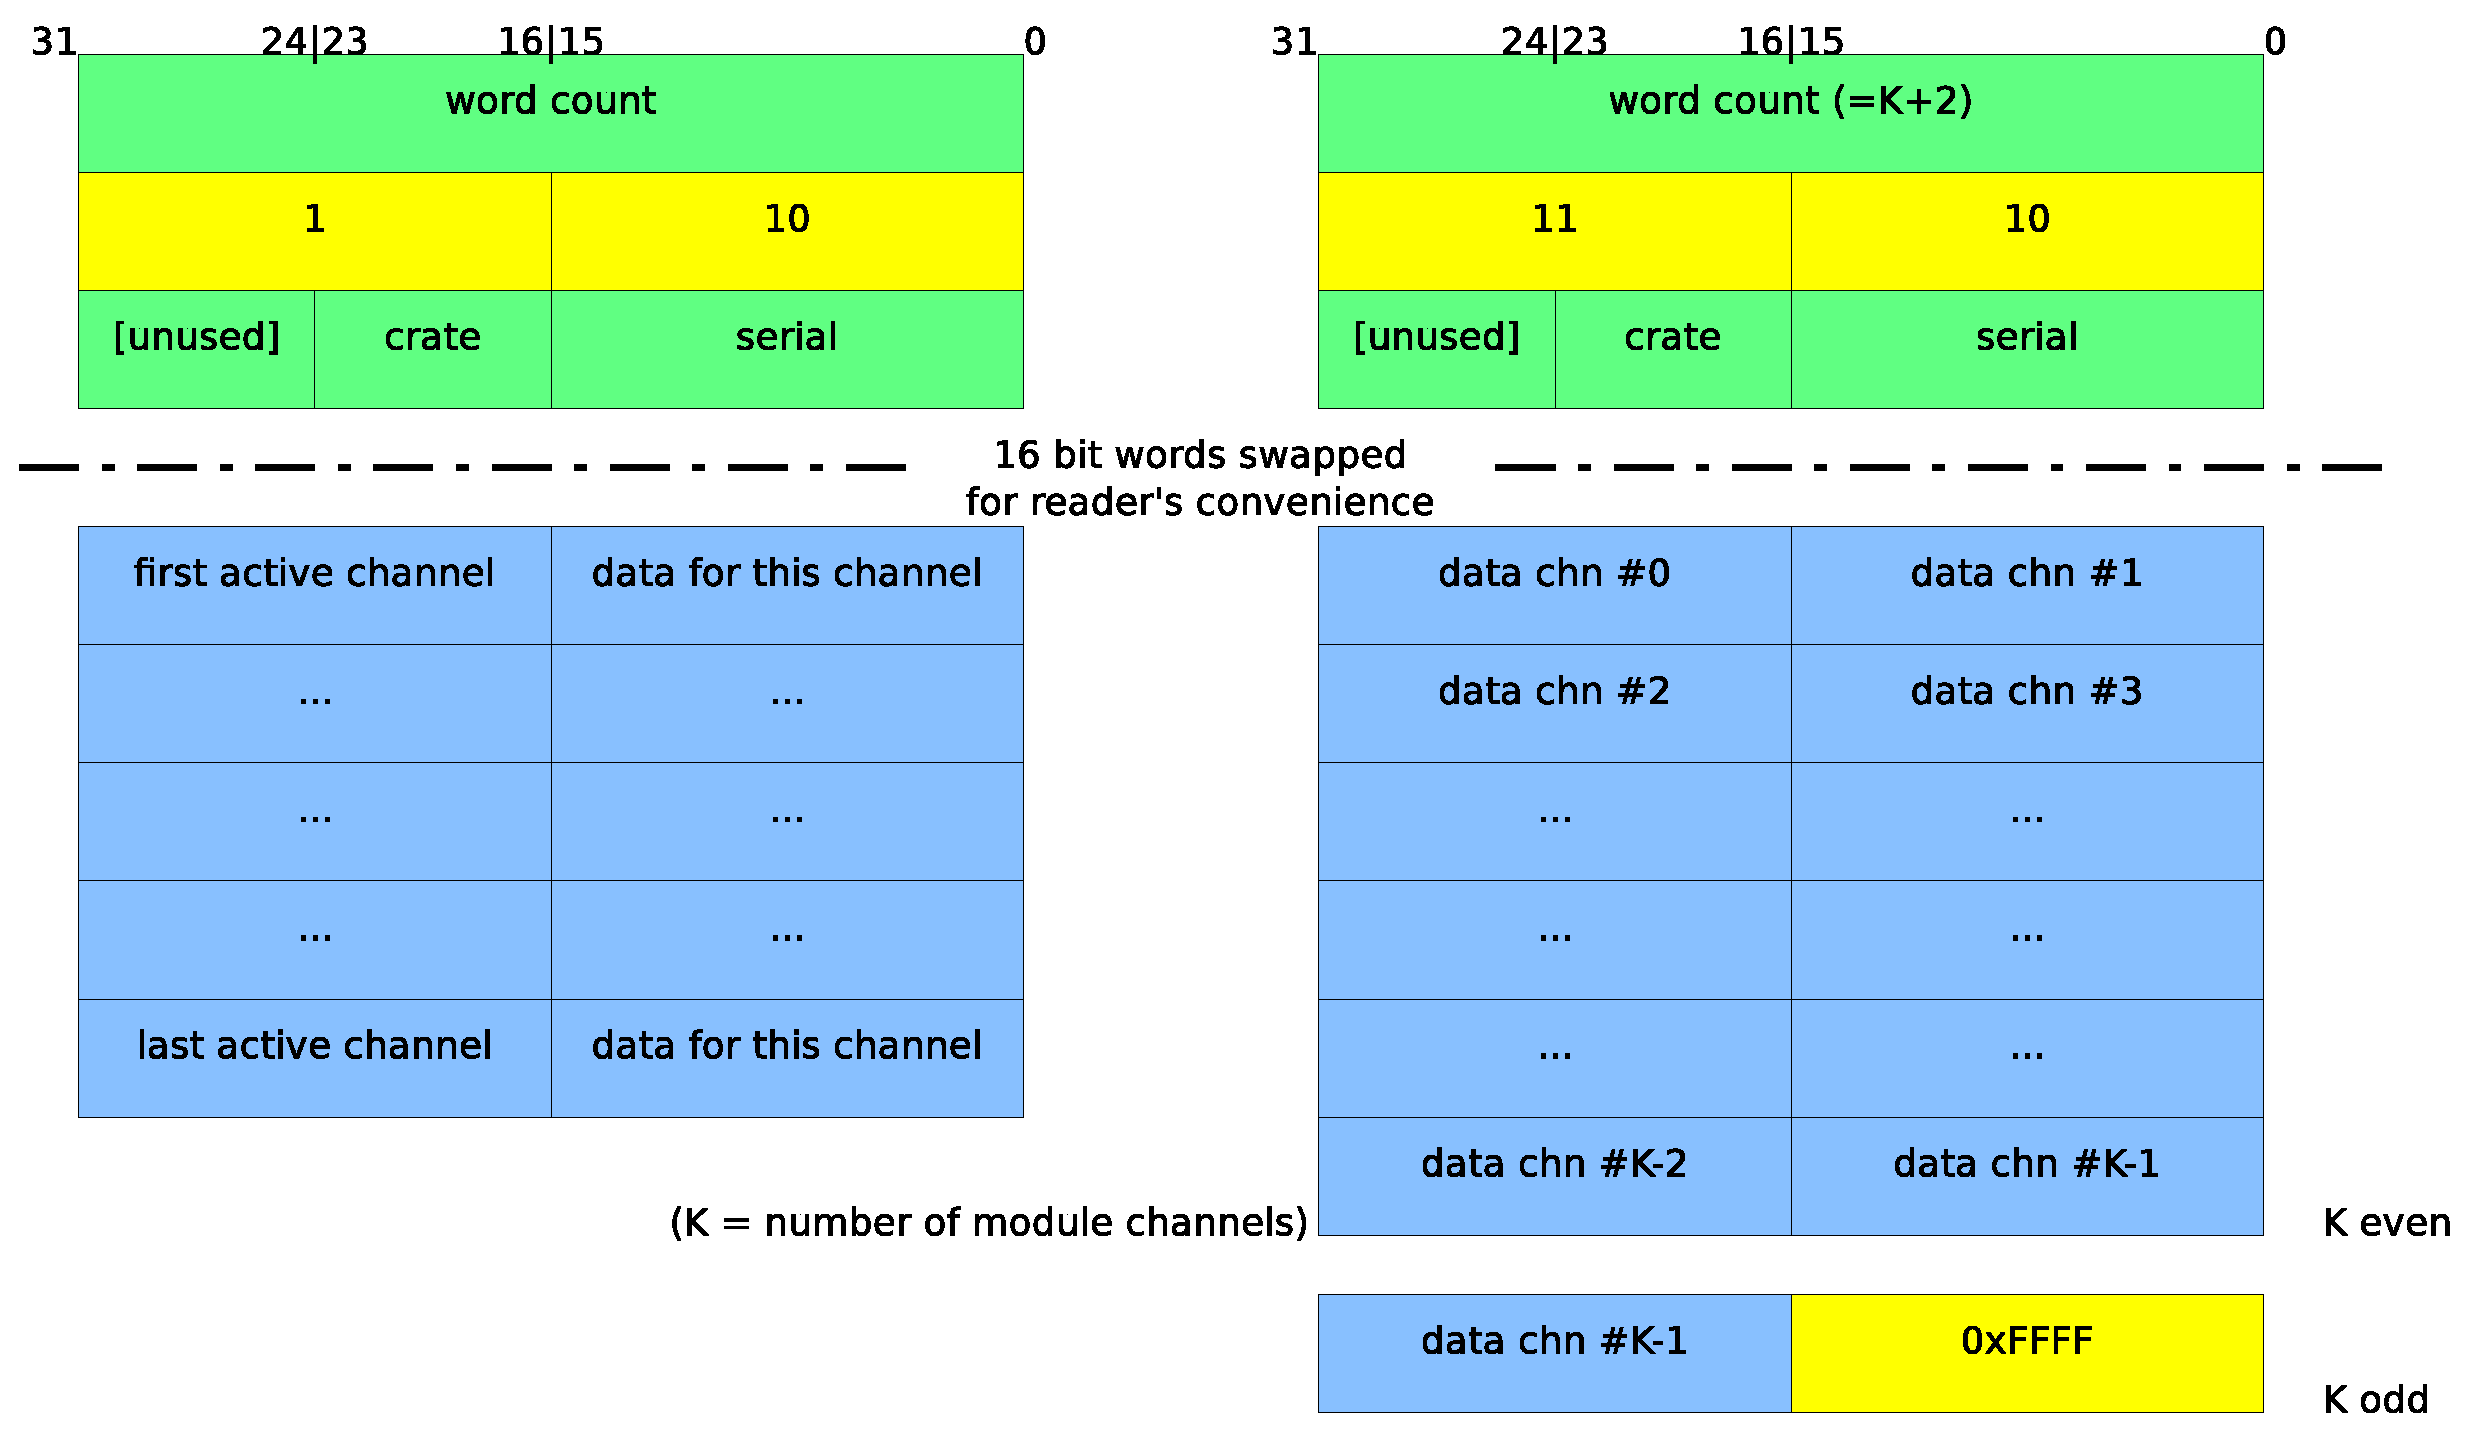
\includegraphics[width=\linewidth]{MedSevt_10_1_11}}
\caption{Subevent formats [10,1] and [10,11]: universal storage}
\label{MedSevt_10_1_11}
\end{figure}
\newpage
\subsection{Multi-module extension: subevent format [10,12]}
Subevent format [10,12] is an extension to format [10,1]: zero-compressed data preceeded by channel
numbers are written together with a module header. Thus several modules may easily be stored in one subevent.
\begin{figure}[H]
\centerline{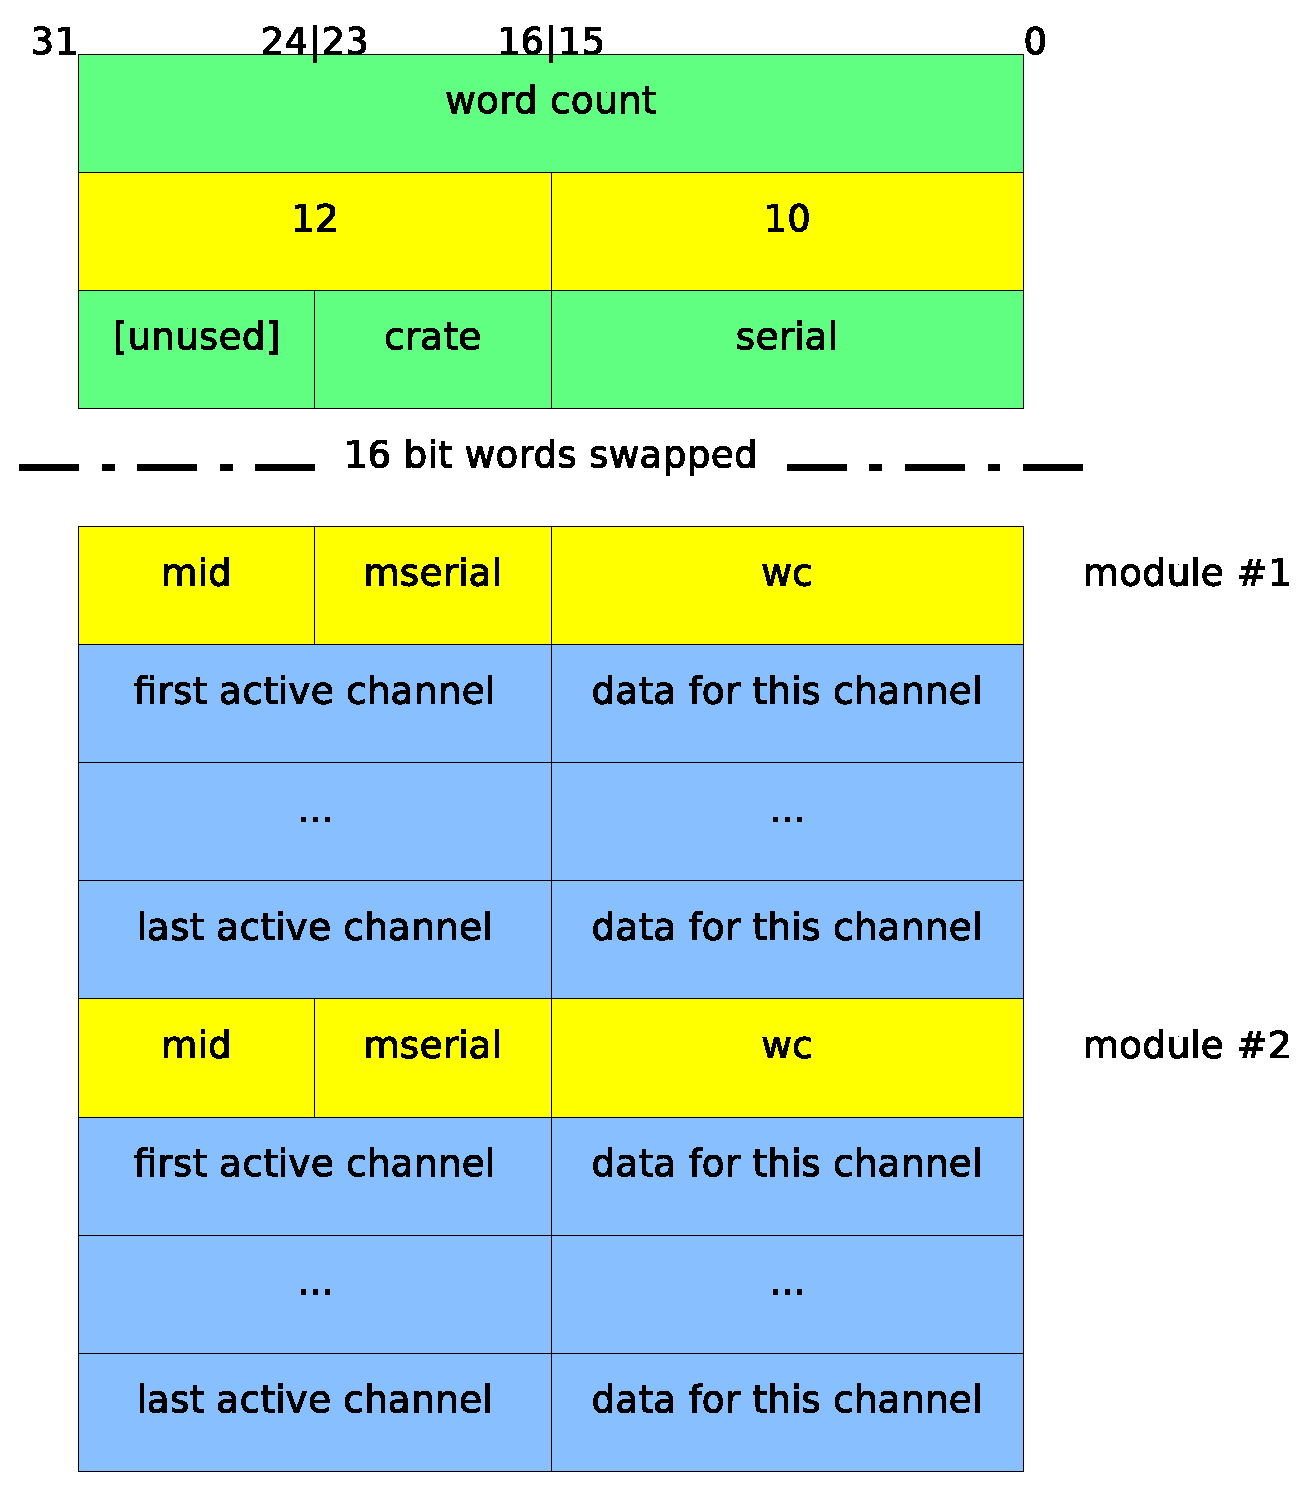
\includegraphics[width=.5\linewidth]{MedSevt_10_12}}
\caption{Subevent format [10,12]: data zero-compressed, any number of modules}
\label{MedSevt_10_12}
\end{figure}
\begin{minipage}{\linewidth}
\begin{table}[H]
\begin{center}
\begin{tabular}{ll}
\hline
\verb+mid+ & module id\\
\verb+mserial+ & module serial number\,\footnote{assigned sequentially during \texttt{Config.C} step} \\
\verb+wc+ & word count, including header words \\
\hline
\end{tabular}
\end{center}
\label{MedSevt_10_12_Legend}
\end{table}
\end{minipage}
\newpage
\subsection{XIA DGF-4C data: subevent formats [10,21], [10,22], and [10,23]}
Formats [10,2X] are used to store original buffers read from XIA DGF-4C modules\,\cite{XIAManuals}.
\begin{figure}[H]
\centerline{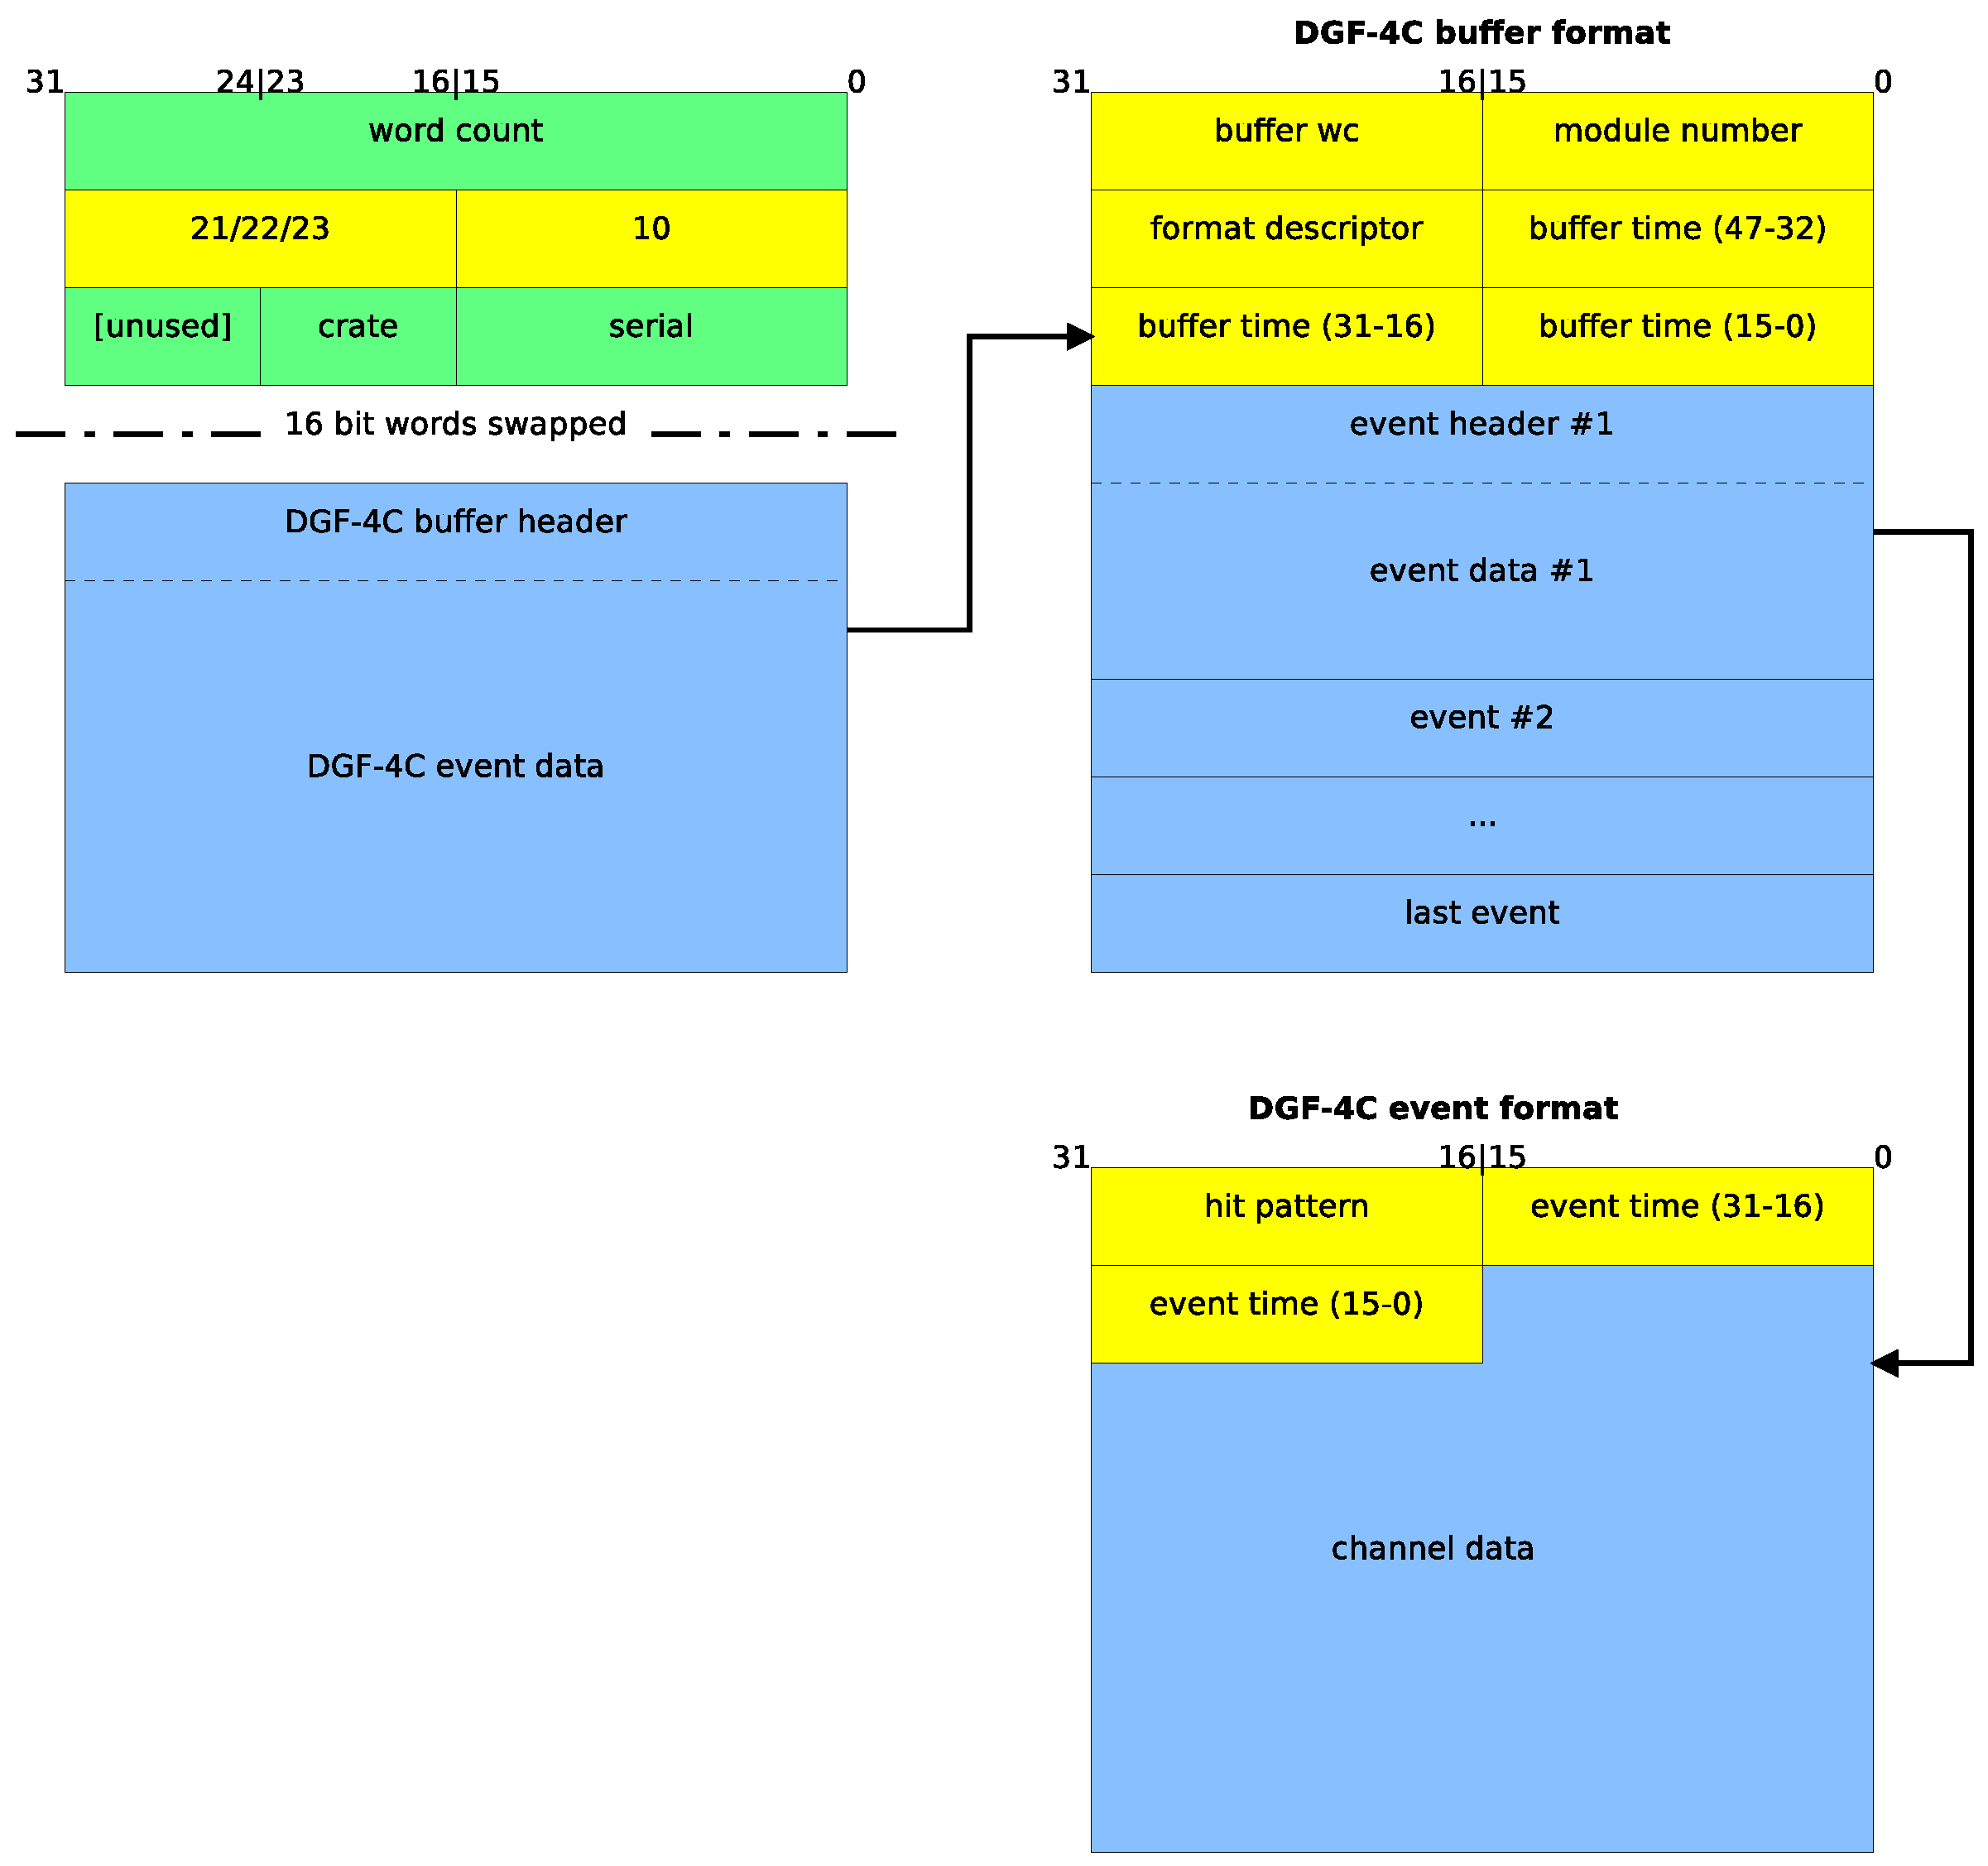
\includegraphics[width=\linewidth]{MedSevt_DGF}}
\caption{Subevent format [10,2X]: DGF-4C buffer data}
\label{MedSevt_DGF}
\end{figure}
\begin{minipage}{\linewidth}
\begin{table}[H]
\begin{center}
\begin{tabular}{ll}
\hline
\multicolumn{2}{c}{buffer header} \\
\hline
\verb+buffer wc+ & number of 16 bit words in this buffer \\
\verb+module number+ & module serial number\,\footnote{assigned sequentially during \texttt{Config.C} step} \\
\verb+format descriptor+ & data format used for channel data \\
\verb+buffer time+ & 48 bit buffer starting time \\
\hline
\multicolumn{2}{c}{event header} \\
\hline
\verb+hit pattern+ & one bit per active channel \\
\verb+event time+ & 32 bit event starting time \\
\hline
\end{tabular}
\end{center}
\label{MedSevt_DGF_Legend}
\end{table}
\end{minipage}
\newpage
Several list mode formats are available to control the DGF-4C data flow. Depending on the value of the format descriptor in
the buffer header (fig.\,\ref{MedSevt_DGF}) long or short channel headers with or without trace data will be written.
Fig.\,\ref{MedSevt_DGF_ChannelFormats} shows different channel layouts.
For a detailed description see\,\cite{XIAManuals}.
\begin{figure}[H]
\centerline{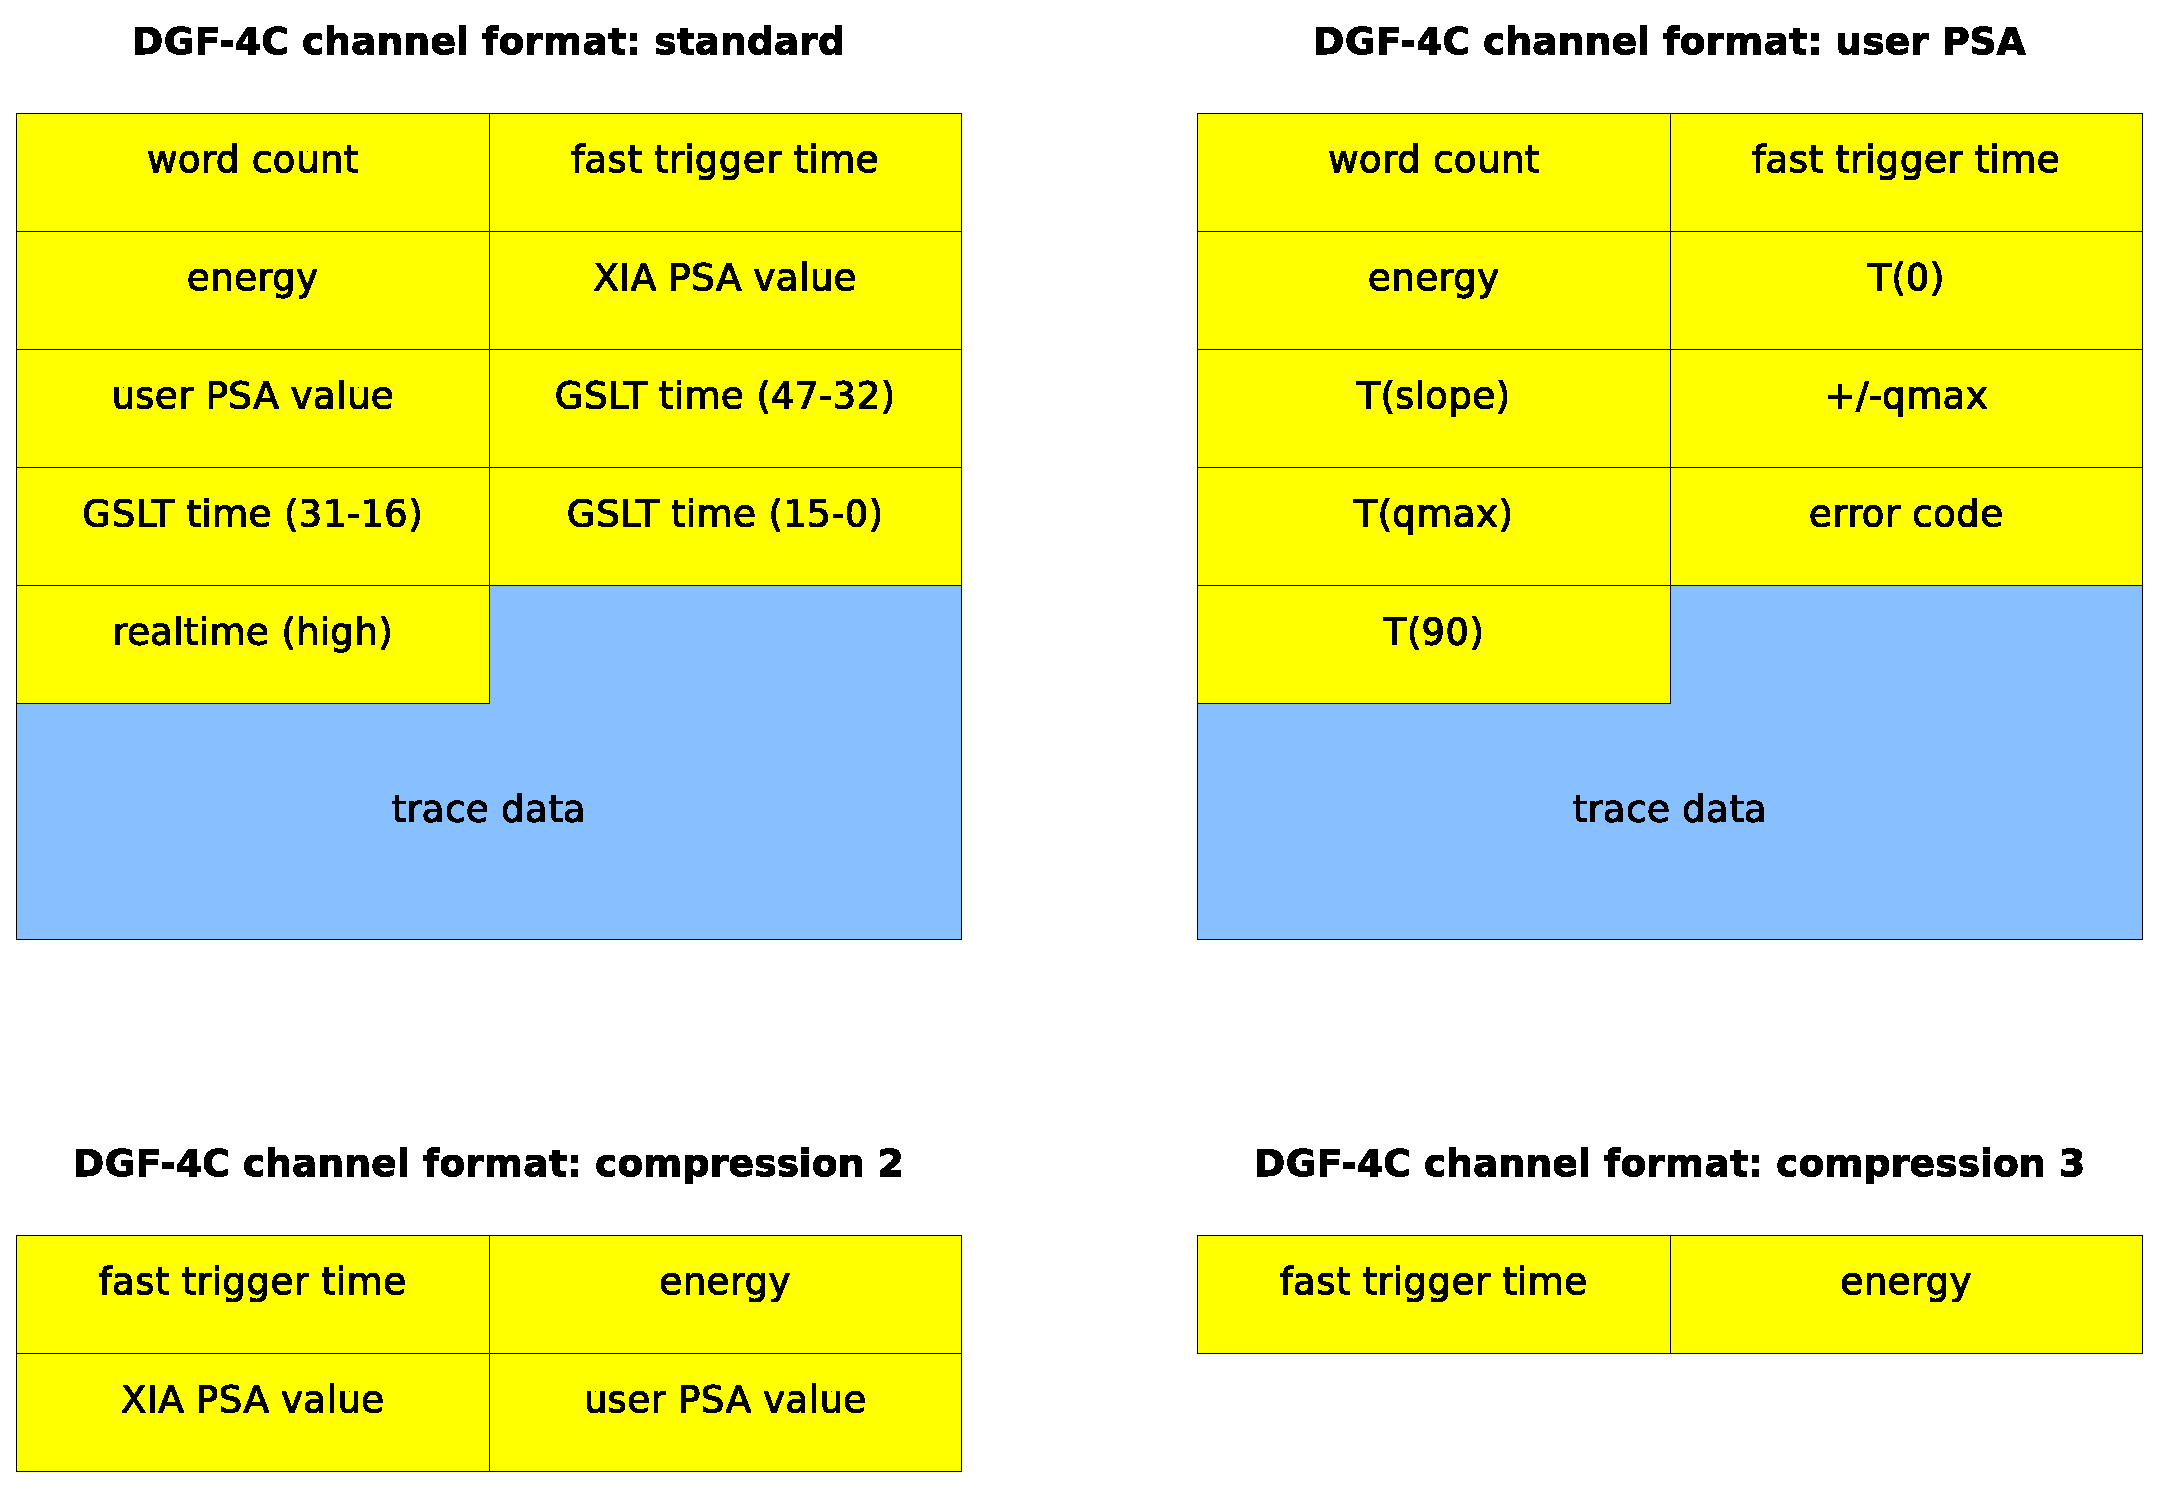
\includegraphics[width=\linewidth]{MedSevt_DGF_ChannelFormats}}
\caption{Subevent format [10,2X]: DGF-4C list mode formats}
\label{MedSevt_DGF_ChannelFormats}
\end{figure}
\begin{minipage}{\linewidth}
\begin{table}[H]
\begin{center}
\begin{tabular}{ll}
\hline
\multicolumn{2}{c}{channel header} \\
\hline
\verb+word count+ & number of 16 bit words written for this channel \\
\verb+fast trigger time+ & time of arrival \\
\verb+energy+ & converted energy value \\
\verb+PSA value+ & result of pulse shape analysis (XIA and user) \\
\verb+GSLT time+ & 48 bit arrival time of global second level trigger \\
\verb+realtime+ & time since last reboot or reset (high word: bits 47-32) \\
\verb+trace data+ & array containing trace data depending on format descriptor \\
\hline
\end{tabular}
\end{center}
\label{MedSevt_DGF_ChannelFormats_Legend}
\end{table}
\end{minipage}
\newpage
\subsection{Silena 4418V/T data: subevent formats [10,31] and [10,32]}
Formats [10,31] and [10,32] are used to store zero-compressed data from Silena 4418V/T modules.
Several modules may be stored in one subevent. In case of uncompressed Silena data subevent type [10,11]
has to be used instead (one module per subevent only).
\begin{figure}[H]
\centerline{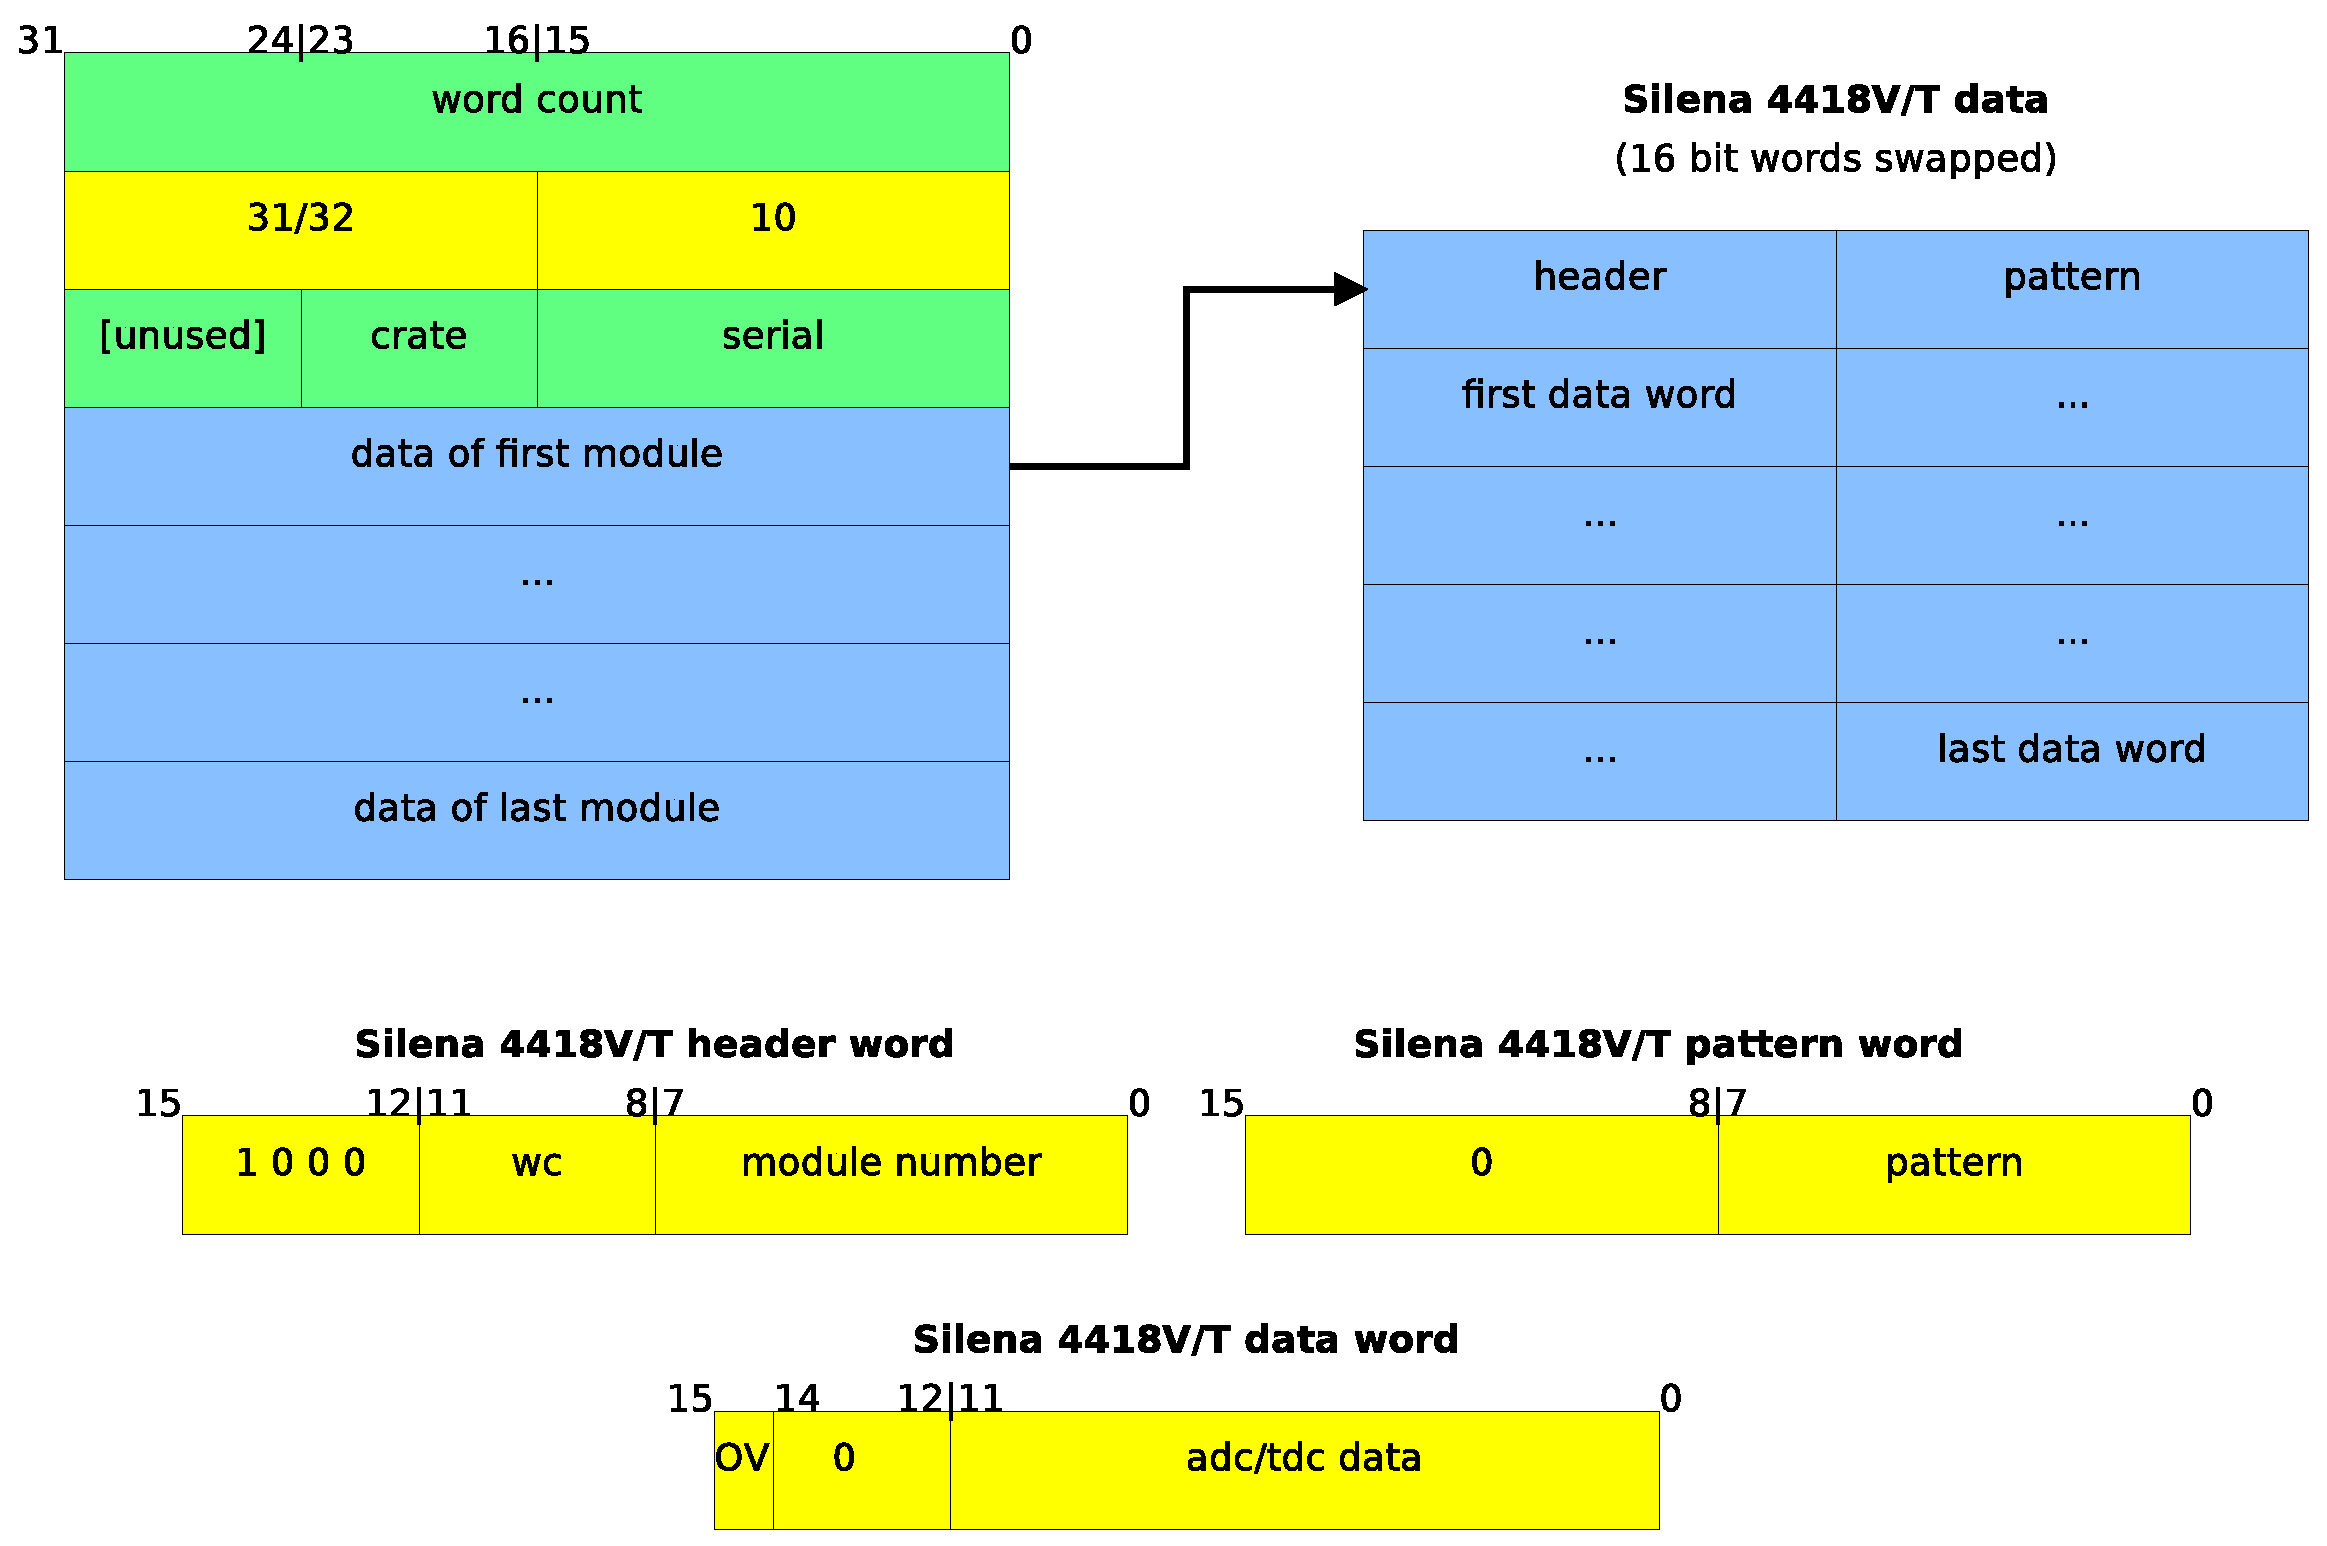
\includegraphics[width=\linewidth]{MedSevt_Silena}}
\caption{Subevent format [10,3X]: Silena 4418V/T data}
\label{MedSevt_Silena}
\end{figure}
\begin{minipage}{\linewidth}
\begin{table}[H]
\begin{center}
\begin{tabular}{ll}
\hline
\verb+wc+ & number of words (including header and pattern) \\
\verb+module number+ & module number\,\footnote{assigned sequentially during \texttt{Config.C} step} \\
\verb+pattern+ & 8 bit pattern word: active channels have bit=1 \\
\verb+data+ & 12 bit adc/tdc data \\
\hline
\end{tabular}
\end{center}
\label{MedSevt_Silena_Legend}
\end{table}
\end{minipage}
\newpage
\subsection{CAEN V7X5 data: subevent formats [10,41], [10,42], and [10,43]}\label{CAEN7X5}
Formats [10,4X] provide containers for original CAEN list mode data produced by modules CAEN V785 and
CAEN V775, respectively. Each CAEN buffer may contain up to 32 events.
In addition, as each event is tagged with module number one may store data from
several CAEN modules in one subevent. To be able to correlate time stamps in
DGF and CAEN branches in MINIBALL experiments data have to be stored one module per subevent, however.
A detailed description of this format may be found in \cite{CAENManual}
\begin{figure}[H]
\centerline{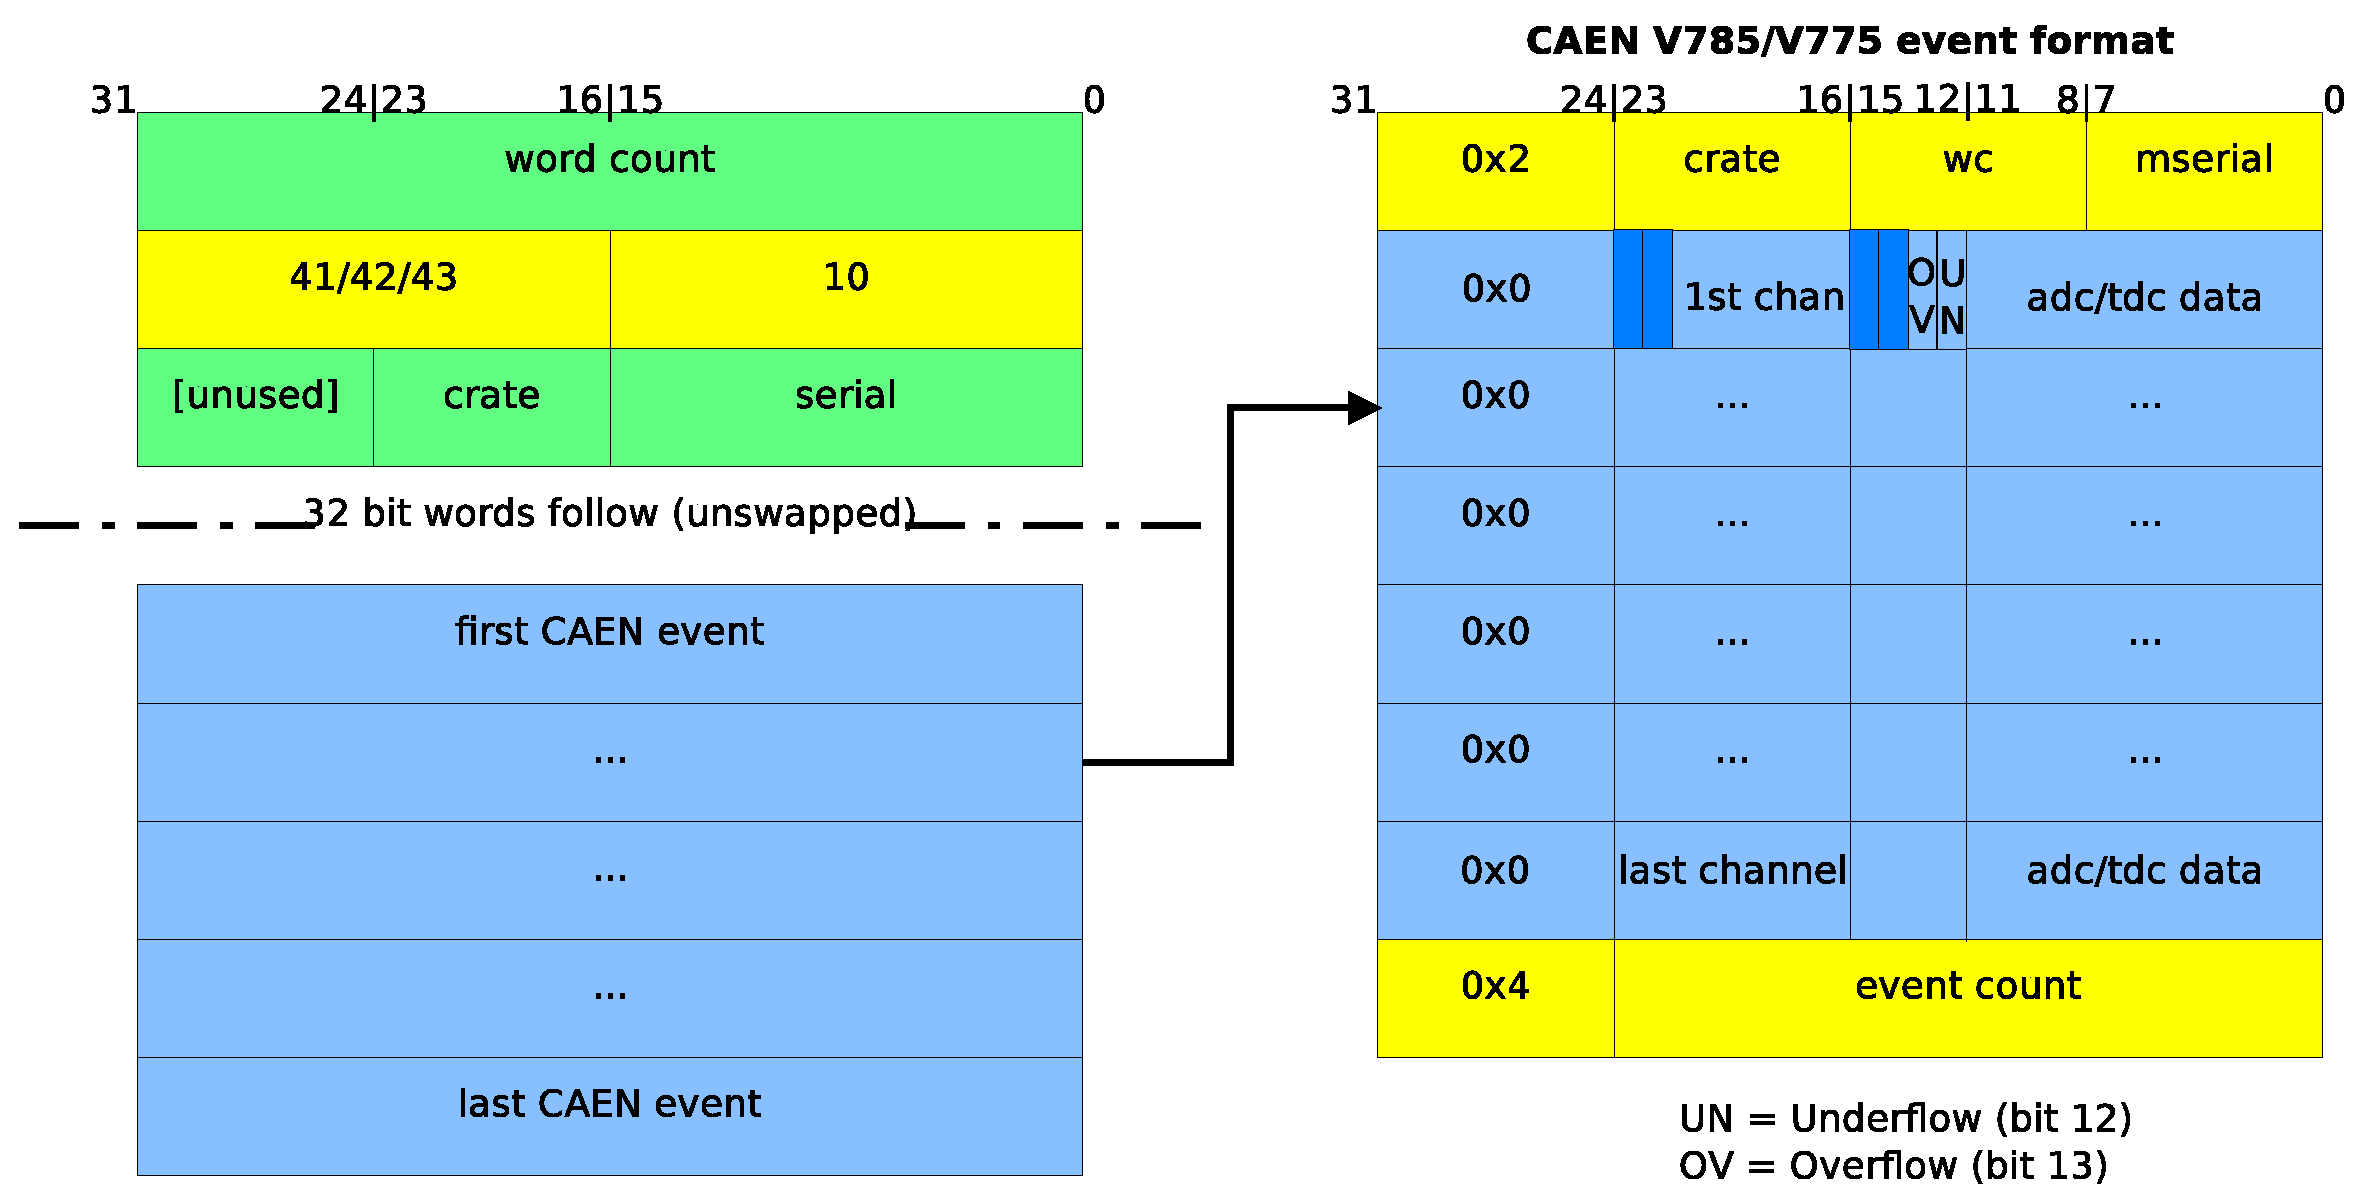
\includegraphics[width=\linewidth]{MedSevt_CAEN_V7X5}}
\caption{Subevent format [10,4X]: CAEN V7X5 ADC/TDC data}
\label{MedSevt_CAEN_7X5}
\end{figure}
\begin{minipage}{\linewidth}
\begin{table}[H]
\begin{center}
\begin{tabular}{ll}
\hline
\verb+0x2+ & header word including word count and module number\,\footnote{GEO address not used} \\
\verb+0x0+ & data word: channel number and converted data\samempfootnote \\
\verb+0x4+ & trailer word: event count\samempfootnote \\
\hline
\verb+crate+ & crate number\,\footnote{currently unused in \MARaBOU{}} \\
\verb+wc+ & number of channel data (32 bit, \underline{excluding} header \& trailer) \\
\verb+mserial+ & module serial number\,\footnote{assigned sequentially during \texttt{Config.C} step} \\
\verb+channel+ & channel number (0 \dots 31) \\
\verb+data+ & 12 bit adc/tdc data + overflow (OV, bit 13) + underflow (UN, bit 12)\\
\verb+event count+ & number of events since last reset \\
\hline
\end{tabular}
\end{center}
\label{MedSevt_CAEN_V7X5_Legend}
\end{table}
\end{minipage}
\newpage
\subsection{CAEN V965 data: subevent format [10,44]}
Format [10,44] provides a container for data produced by a CAEN V965 QDC.
It is very similar to formats [10,4X] described in \ref{CAEN7X5}. As the qdc module integrates twice for each input there may be two
data words per channel. The range bit then denotes whether it is the low (fine gain) or high (coarse gain) integration.
\begin{figure}[H]
\centerline{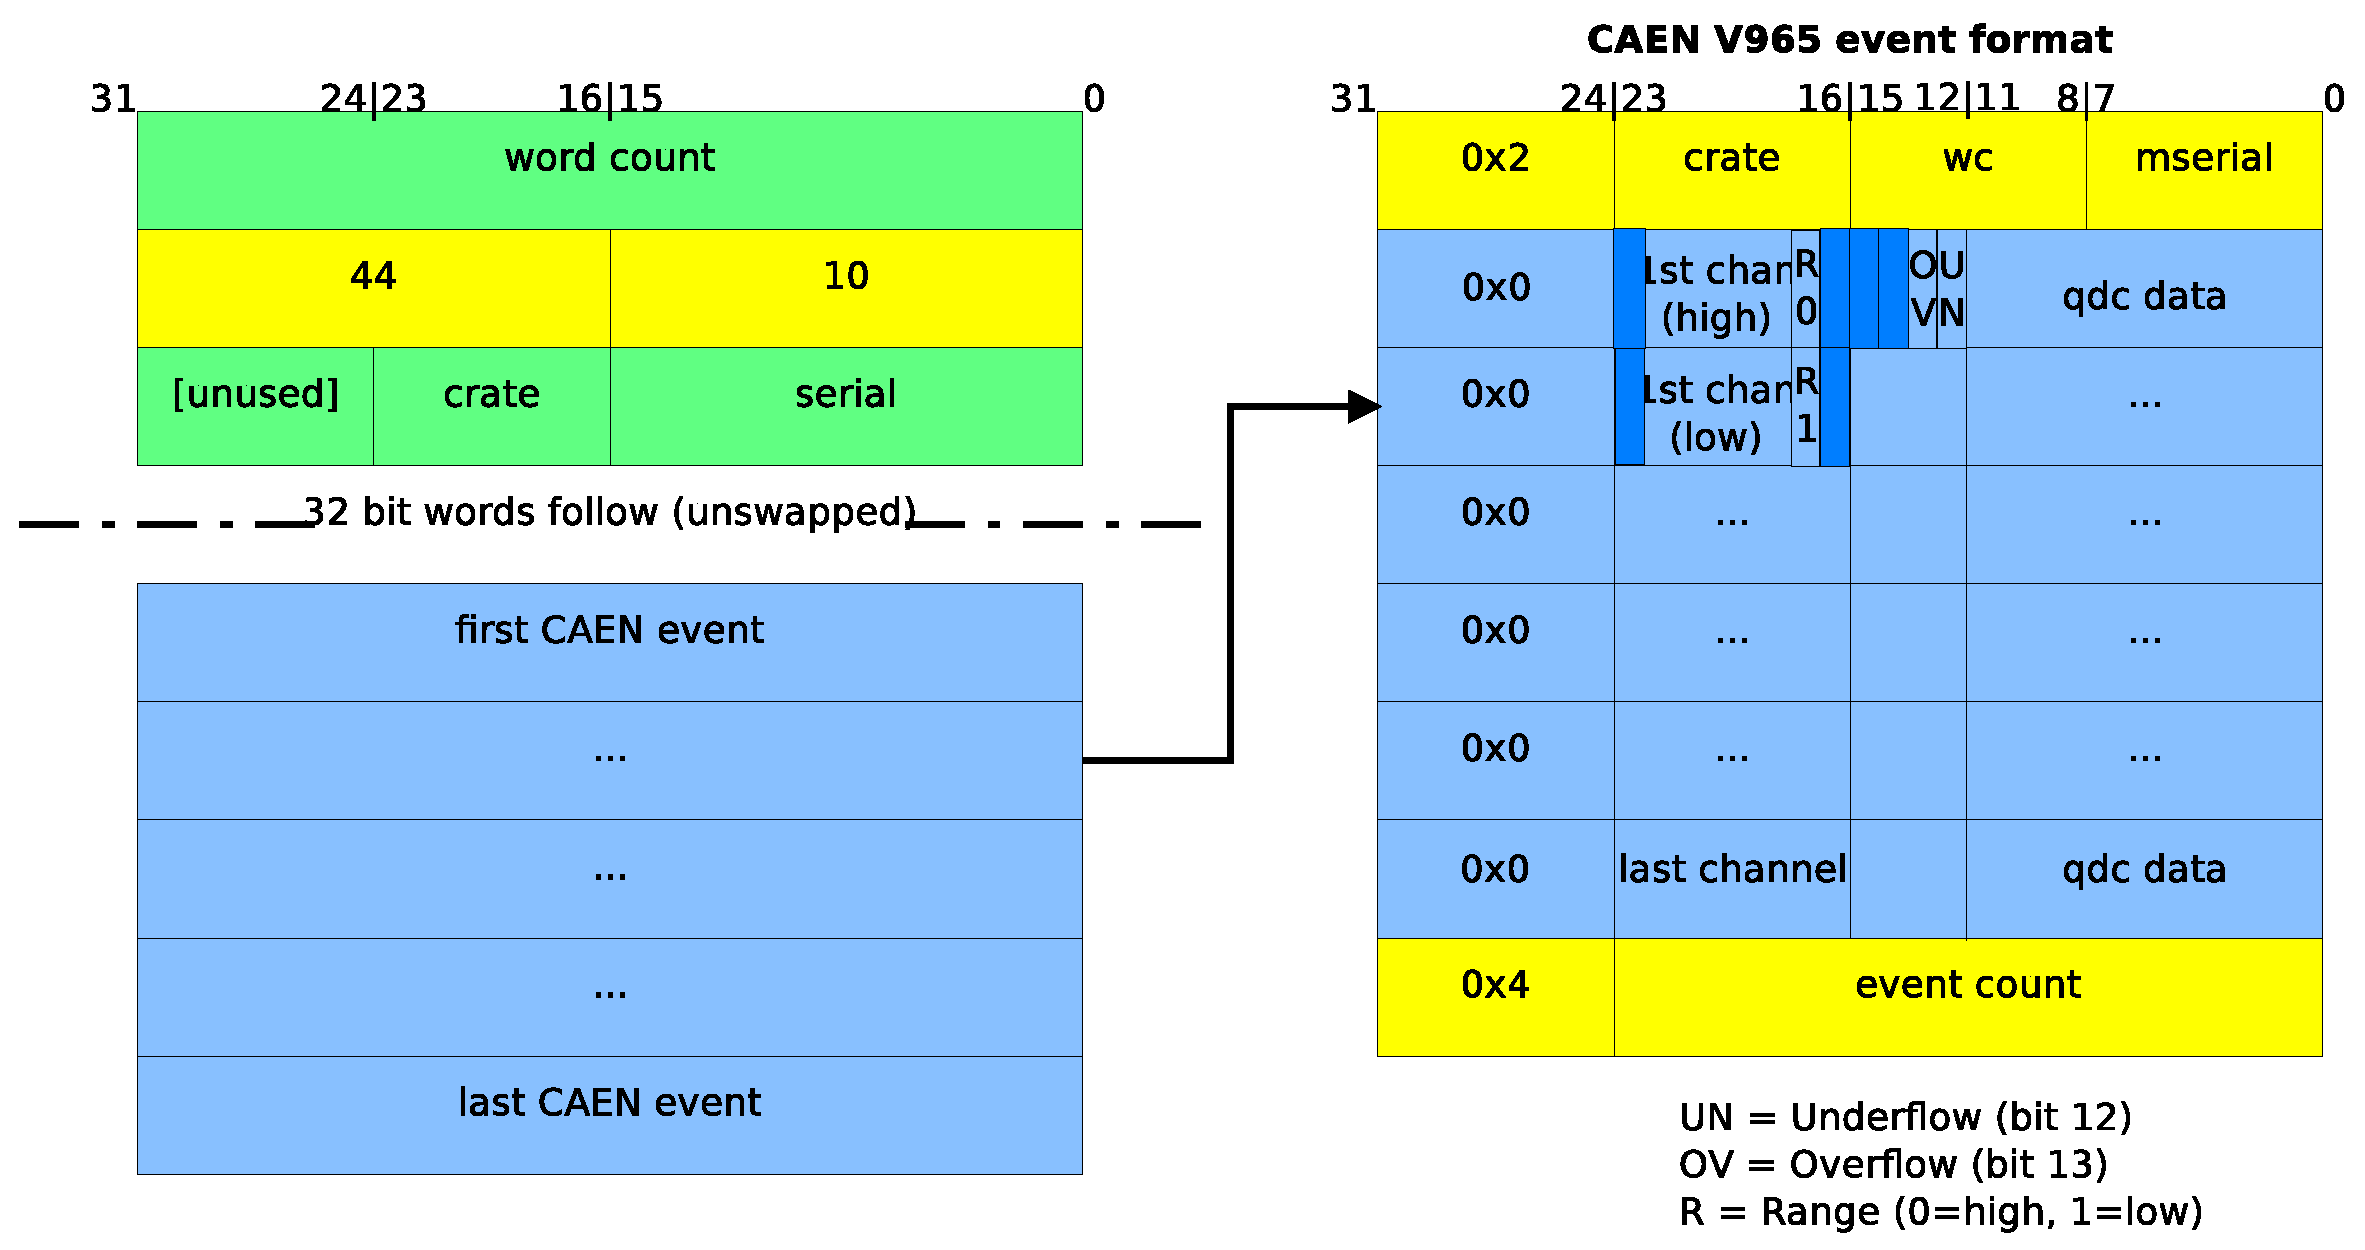
\includegraphics[width=\linewidth]{MedSevt_CAEN_V965}}
\caption{Subevent format [10,44]: CAEN V965 QDC data}
\label{MedSevt_CAEN_V965}
\end{figure}
\begin{minipage}{\linewidth}
\begin{table}[H]
\begin{center}
\begin{tabular}{ll}
\hline
\verb+0x2+ & header word including word count and module number\,\footnote{GEO address not used} \\
\verb+0x0+ & data word: channel number and converted data\samempfootnote \\
\verb+0x4+ & trailer word: event count\samempfootnote \\
\hline
\verb+crate+ & crate number\,\footnote{currently unused in \MARaBOU{}} \\
\verb+wc+ & number of channel data (32 bit, \underline{excluding} header \& trailer) \\
\verb+mserial+ & module serial number\,\footnote{assigned sequentially during \texttt{Config.C} step} \\
\verb+channel+ & channel number (V965A: 0 \dots 7, V965: 0 \dots 15) + range bit (bit 17)\\
\verb+data+ & 12 bit adc/tdc data + overflow (OV, bit 13) + underflow (UN, bit 12)\\
\verb+event count+ & number of events since last reset \\
\hline
\end{tabular}
\end{center}
\label{MedSevt_CAEN_V965_Legend}
\end{table}
\end{minipage}
\newpage
\subsection{SIS 3XXX data: subevent formats [10,51], [10,52], and [10,53]}
Formats [10,5X] are designed to store data produced by SIS 3600 or SIS 3801 modules.
This format is identical to format [10,12].
\begin{figure}[H]
\centerline{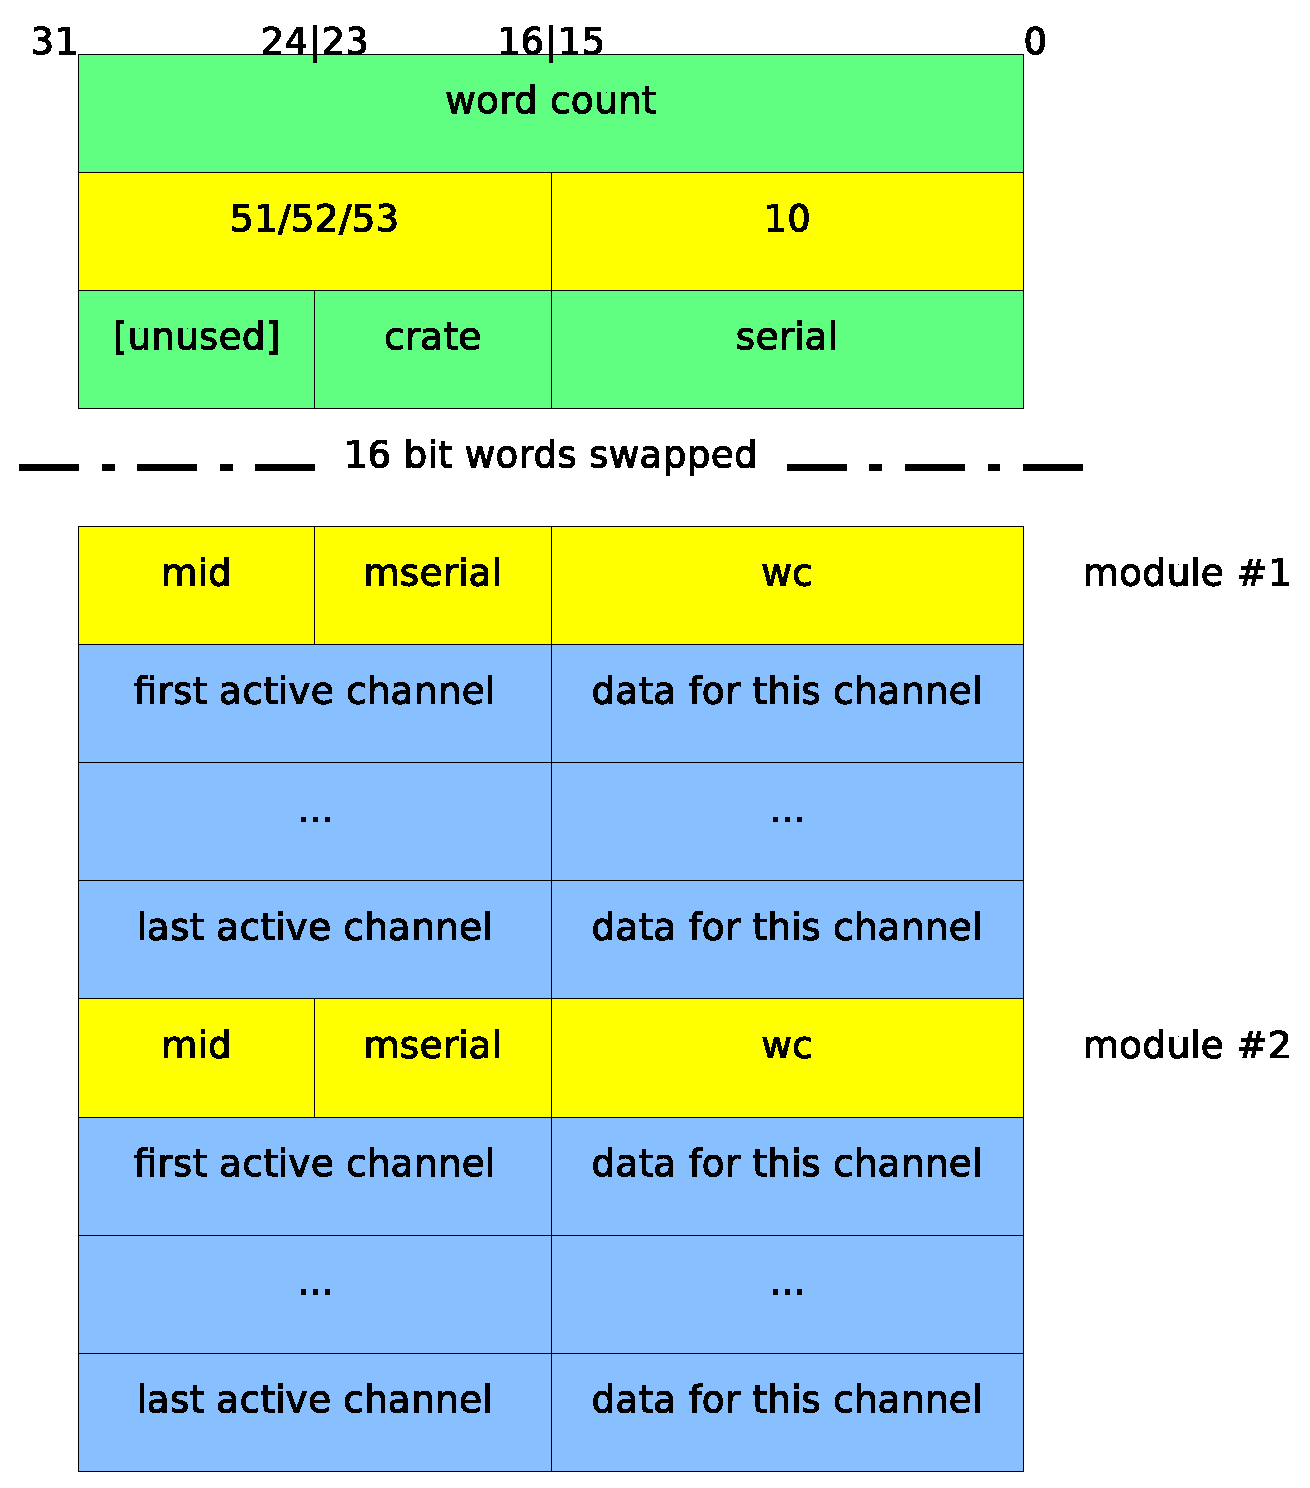
\includegraphics[width=.5\linewidth]{MedSevt_SIS}}
\caption{Subevent format [10,5X]: SIS 3XXX data}
\label{MedSevt_SIS}
\end{figure}
\begin{minipage}{\linewidth}
\begin{table}[H]
\begin{center}
\begin{tabular}{ll}
\hline
\verb+mid+ & module id\\
\verb+mserial+ & module serial number\,\footnote{assigned sequentially during \texttt{Config.C} step} \\
\verb+wc+ & word count, including header words \\
\hline
\end{tabular}
\end{center}
\label{MedSevt_SIS_Legend}
\end{table}
\end{minipage}
\vspace{5mm}\\
Note: In current MINIBALL experiments data from
SIS 3801 scalers will be written using format [10,11] rather than this one.
\newpage
\subsection{Plain data containers: subevent formats [10,91], 10,92], and [10,93]}
Formats [10,9X] provide containers to store data that are not directly related to a hardware module
(e.g. internal DGF scalers).
There are containers for short [10,91], long [10,92], and float items [10,93], respectively.
\begin{figure}[H]
\centerline{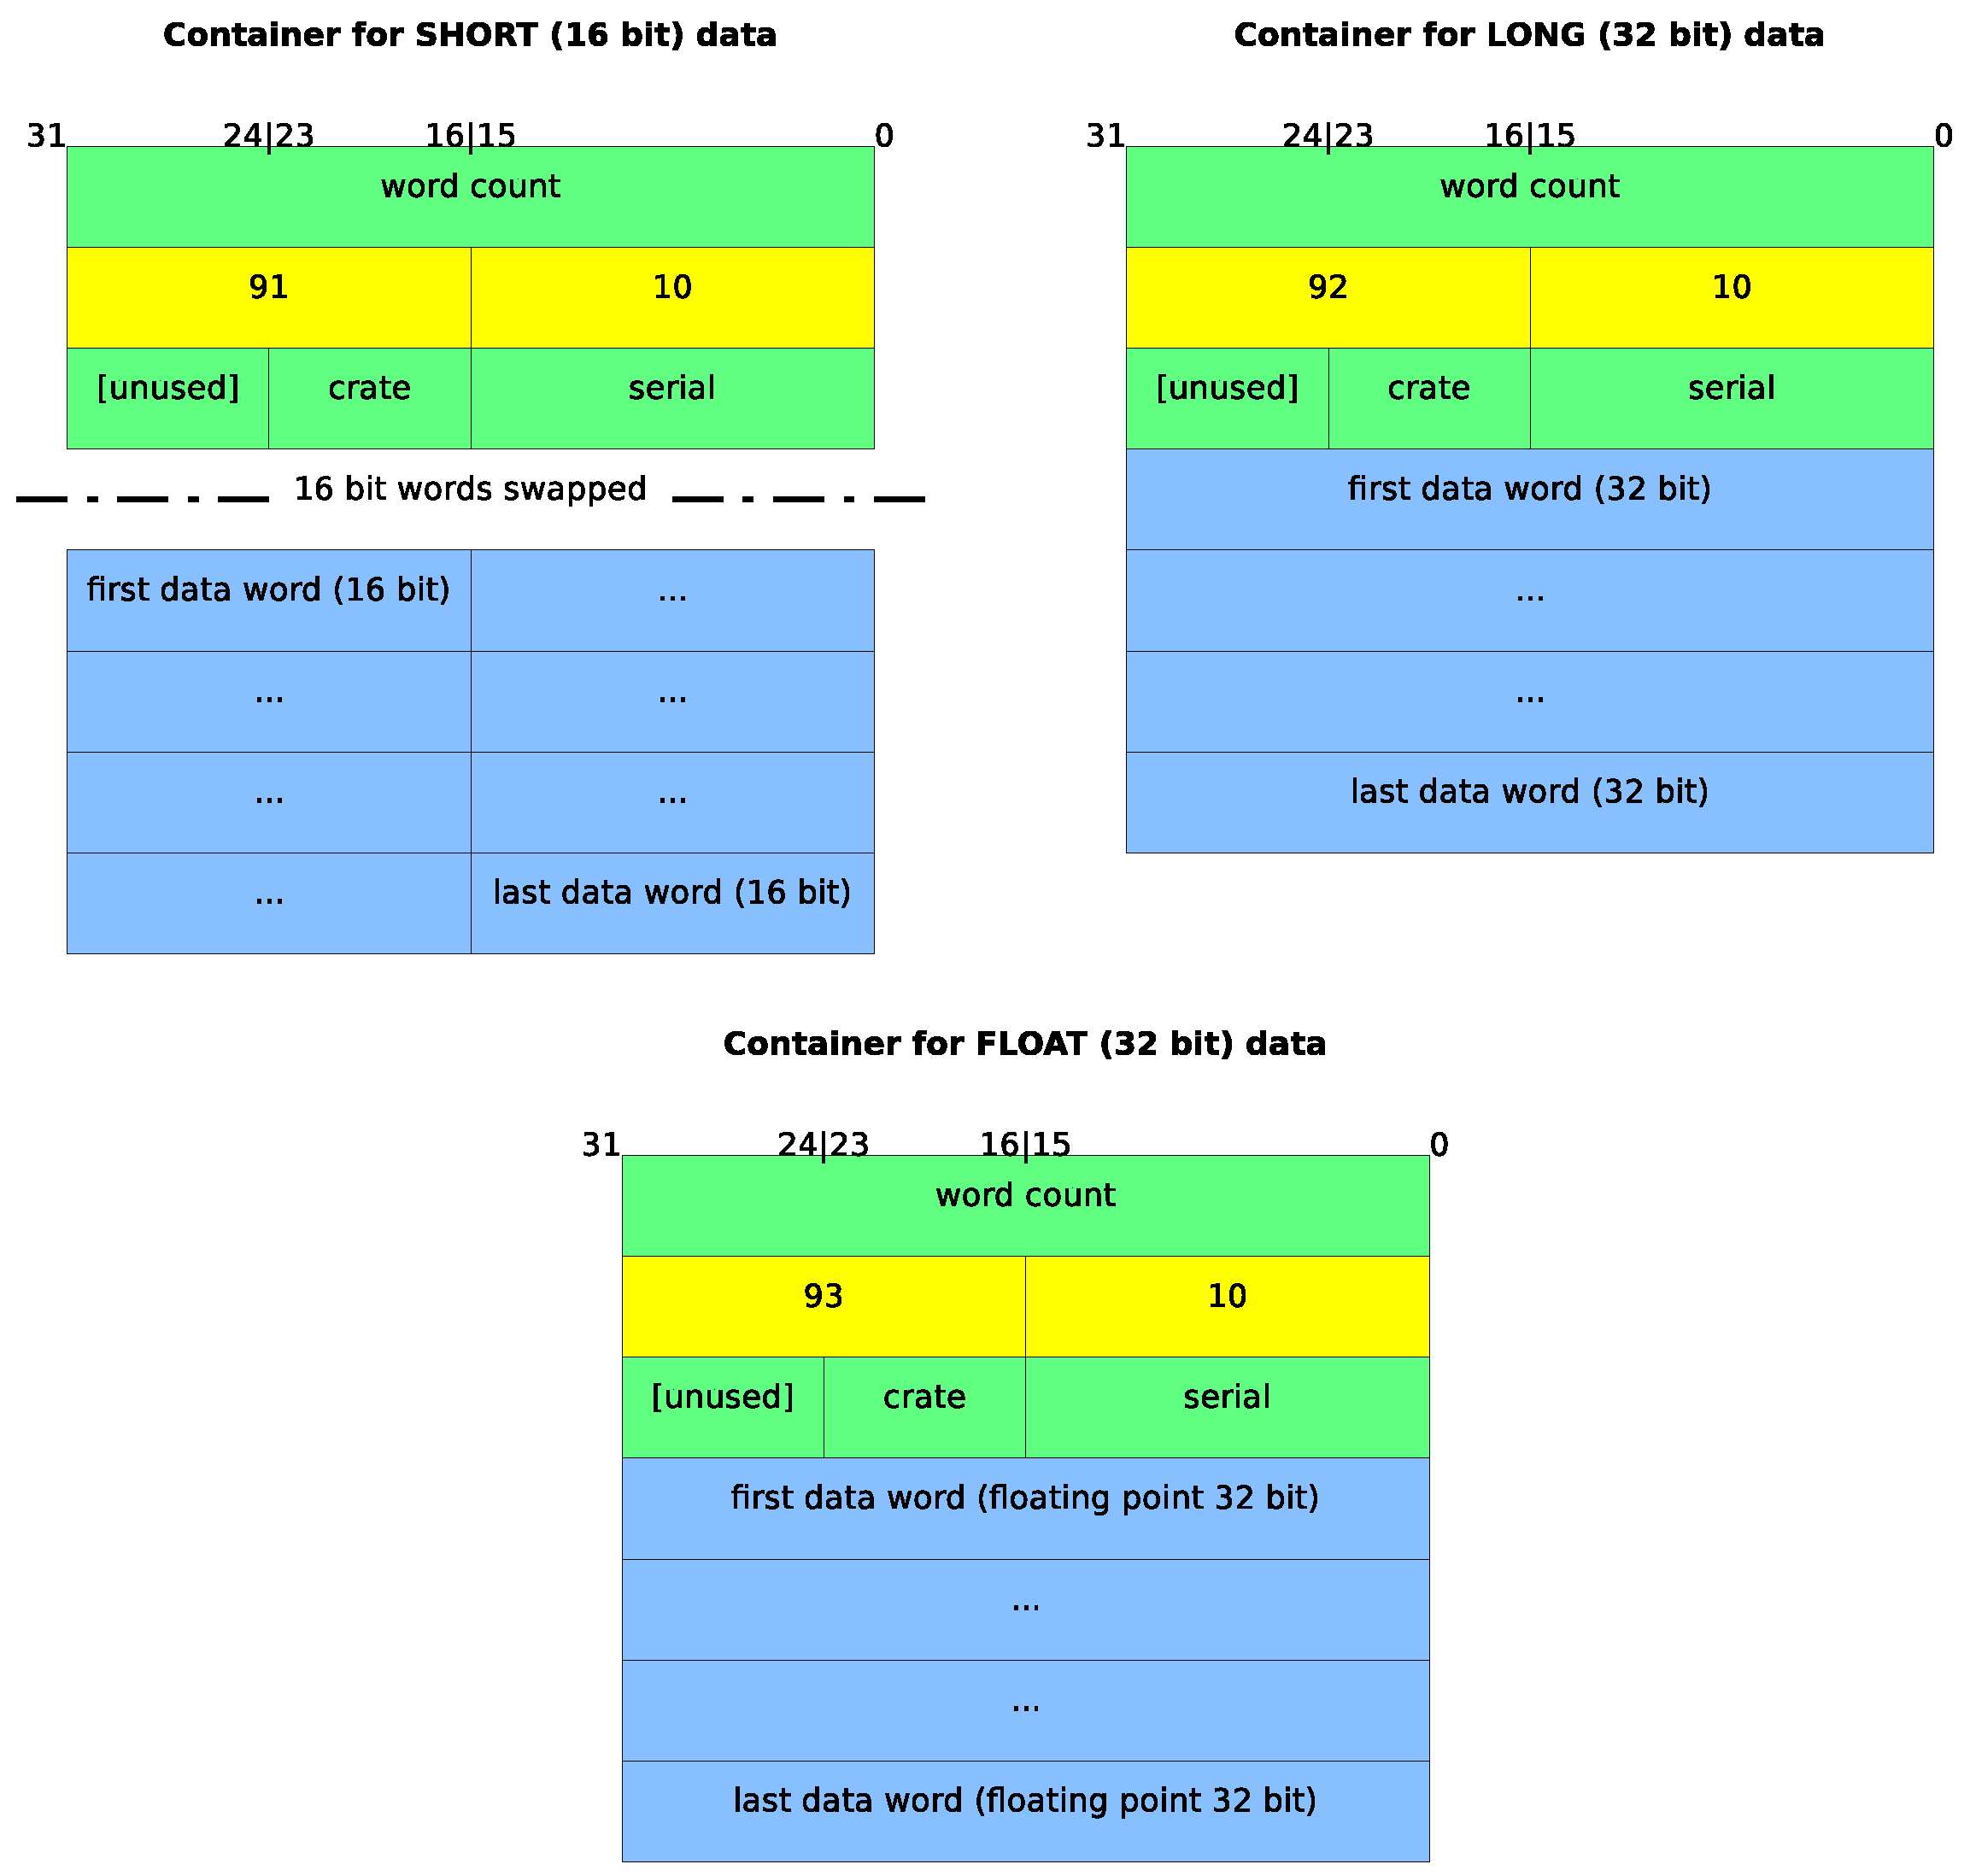
\includegraphics[width=\linewidth]{MedSevt_Data_X}}
\caption{Subevent format [10,9X]: Plain data containers}
\label{MedSevt_Data_X}
\end{figure}
\newpage
\section{User Interface to MED data (C API)}
This section describes the C user interface which may be used to access MED data without running ROOT.
It includes function calls to
\begin{itemize}
	\item	open med files
	\item	read event by event and dispatch over event trigger
	\item	decode subevent header
	\item	extract subevent data and dispatch over subevent type and/or serial number
\end{itemize}
Any prototype for this user interface is defined in file \verb+mbsio.h+.
So you have to include this file in front of your code:
\begin{center}
\begin{blueboxed}{.3\linewidth}
	\verb+#include <stdio.h>+\\
	\verb+#include "mbsio.h"+
\end{blueboxed}
\end{center}
To include this package in a \texttt{C++} environment, add prototype definitions from file \verb+mbsio_protos.h+:\hfill
\begin{center}
\begin{blueboxed}{.3\linewidth}
	\verb+#include "mbsio_protos.h"+
\end{blueboxed}
\end{center}\vspace{5mm}
\subsection{Open a \texttt{.med} file}\vspace{3mm}
\begin{blueboxed}{\linewidth}
	\verb+MBSDataIO * mbs_open_file(const char * FileName, const char * Connect,+\\
	\verb+                                                 int BufSize, FILE * HdrOut);+\\
	\verb+int mbs_close_file(MBSDataIO * MbsHandle);+
\end{blueboxed}
\begin{center}
\begin{tabular}{ll}
\verb+const char * FileName+	& file name, extension has to be \verb+.med+\\
\verb+const char * Connect+	& how to connect to med data stream, has to be \verb+F+ ("File")\\
\verb+int BufSize+		& buffer size, normally \verb+0x4000+ (16k)\\
\verb+FILE * HdrOut+		& where to output header info, set to \verb+NULL+ for "no output"\\
\verb+MBSDataIO * MbsHandle+	& file handle to access med data\\
\end{tabular}
\end{center}
\blue{mbs\_open\_file} opens a med raw data file for reading and returns a file handle to refer to it.

\blue{mbs\_close\_file} closes the file pointed to by the file handle.
\vspace{5mm}

\begin{yellowboxed}{\linewidth}
Example:\\
\verb+            MBSDataIO * mbsHandle;+\\
\verb+            mbsHandle = mbs_open_file("run123.med", "F", 0x4000, NULL);+\\
\verb+            if (mbsHandle = NULL) { printf("Error\n"); exit(1); }+\\
\end{yellowboxed}\vspace{5mm}
\newpage
\subsection{Read event by event and dispatch over event trigger}\vspace{3mm}
\begin{center}
\begin{blueboxed}{.7\linewidth}
	\verb+unsigned int mbs_next_event(MBSDataIO * MbsHandle);+\\
	\verb+int mbs_get_event_trigger(MBSDataIO * MbsHandle);+
\end{blueboxed}
\end{center}
\begin{center}
\begin{tabular}{ll}
\verb+MBSDataIO * MbsHandle+	& file handle as returned by \verb+mbs_open_file+\\
\end{tabular}
\end{center}
\blue{mbs\_next\_event} moves on to next event, adjusts internal pointers.
Returns event type \verb+[subtype,type]+ which is always \verb+[1,10]+.
User has to check for special return values \verb+MBS_ETYPE_EOF+ (end of file),
\verb+MBS_ETYPE_ERROR+ (error), and \verb+MBS_ETYPE_ABORT+ (abort).

\blue{mbs\_get\_event\_trigger} returns trigger number of current event.
\vspace{5mm}

\begin{yellowboxed}{\linewidth}
Example:\\
\verb+            unsigned int evtType;+\\
\verb+            int evtTrigger;+\\
\verb+            while (1) {+\\
\verb+                evtType = mbs_next_event(mbsHandle);+\\
\verb+                if (evtType == MBS_ETYPE_EOF) {+\\
\verb+                      printf("End of file\n");+\\
\verb+                      mbs_close_file(mbsHandle);+\\
\verb+                } else if (evtType == MBS_ETYPE_ERROR) {+\\
\verb+                      printf("Illegal event - skipped\n");+\\
\verb+                      continue;+\\
\verb+                } else if (evtType == MBS_ETYPE_ABORT) {+\\
\verb+                      printf("Illegal event - aborting\n");+\\
\verb+                      break;+\\
\verb+                } else {+\\
\verb+                      evtTrigger = mbs_get_event_trigger(mbsHandle);+\\
\verb+                      switch (evtTrigger) {+\\
\verb+                          case kMrbTriggerStartAcquisition:+\\
\verb+                               printf("Trigger \"start acquisition\"\n");+\\
\verb+                               break;+\\
\verb+                          case kMrbTriggerStopAcquisition:+\\
\verb+                               printf("Trigger \"stop acquisition\"\n");+\\
\verb+                               break;+\\
\verb+                          case kMrbTriggerReadout:+\\
\verb+                               process_event(mbsHandle, evtTrigger);+\\
\verb+                               break;+\\
\verb+                          case .....+\\
\verb+                               break;+\\
\verb+                          default:+\\
\verb+                               printf("Illegal trigger %d\n", evtTrigger);+\\
\verb+                               break;+\\
\verb+                      }+
\verb+                  }+\\
\verb+             }+
\end{yellowboxed}
\newpage
\subsection{Decode subevent header}\vspace{3mm}
\begin{center}
\begin{blueboxed}{.8\linewidth}
	\verb+unsigned int mbs_next_sheader(MBSDataIO * MbsHandle);+\\
	\verb+unsigned int mbs_get_sevent_subtype(MBSDataIO * MbsHandle);+\\
	\verb+int mbs_get_sevent_serial(MBSDataIO * MbsHandle);+
\end{blueboxed}
\end{center}
\begin{center}
\begin{tabular}{ll}
\verb+MBSDataIO * MbsHandle+	& file handle as returned by \verb+mbs_open_file+\\
\end{tabular}
\end{center}
\blue{mbs\_next\_sheader} moves on to next subevent of current event.
Decodes header information and returns subevent type \verb+[subtype,type]+.
User has to check for special return values \verb+MBS_STYPE_EOE+ (end of event),
\verb+MBS_STYPE_ERROR+ (error), and \verb+MBS_STYPE_ABORT+ (abort).

\blue{mbs\_get\_sevent\_subtype} returns subtype portion of subevent type (LH word of \verb+[subtype,type]+, right-shifted).

\blue{mbs\_get\_sevent\_serial} returns serial number of current subevent.

Subevent type and/or serial number may then be used to dispatch to different decoding routines.
\vspace{5mm}

\begin{yellowboxed}{\linewidth}
Example:\\
\verb+            void process_event(MBSDataIO * mbsHandle, int evtTrigger) {+\\
\verb+                unsigned int sevtType;+\\
\verb+                int sevtSerial;+\\
\verb+                while (1) {+\\
\verb+                    sevtType = mbs_next_sheader(mbsHandle);+\\
\verb+                    if (sevtType == MBS_STYPE_EOE) {+\\
\verb+                        return;+\\
\verb+                    } else if (sevtType == MBS_STYPE_ERROR) {+\\
\verb+                        printf("Illegal subevent - skipped\n");+\\
\verb+                        continue;+\\
\verb+                    } else if (sevtType == MBS_STYPE_ABORT) {+\\
\verb+                        printf("Illegal subevent - aborting\n");+\\
\verb+                        break;+\\
\verb+                    } else {+\\
\verb+                        sevtSerial = mbs_get_sevent_serial(mbsHandle);+\\
\verb+                        process_subevent(mbsHandle, sevtSerial);+\\
\verb+                    }+\\
\verb+                }+\\
\verb+            }+
\end{yellowboxed}
\newpage
\subsection{Extract subevent data, dispatch over subevent serial and/or type}\vspace{3mm}
\begin{center}
\begin{blueboxed}{.8\linewidth}
	\verb+unsigned int mbs_next_sdata(MBSDataIO * MbsHandle);+\\
	\verb+int mbs_get_sevent_wc(MBSDataIO * MbsHandle);+\\
	\verb+unsigned short * mbs_get_sevent_dataptr(MBSDataIO * MbsHandle);+
\end{blueboxed}
\end{center}
\begin{center}
\begin{tabular}{ll}
\verb+MBSDataIO * MbsHandle+	& file handle as returned by \verb+mbs_open_file+\\
\end{tabular}
\end{center}
\blue{mbs\_next\_sdata} moves on to data section of current subevent, adjusts pointers.
Returns subevent type \verb+[subtype,type]+.
User has to check for special return values 
\verb+MBS_STYPE_ERROR+ (error) and \verb+MBS_STYPE_ABORT+ (abort).

\blue{mbs\_get\_sevent\_wc} returns word count of current subevent (16 bit words).

\blue{mbs\_get\_sevent\_dataptr} returns pointer to first data word.
\vspace{5mm}

\begin{yellowboxed}{\linewidth}
Example:\\
\verb+            void process_subevent(MBSDataIO * mbsHandle, int sevtSerial) {+\\
\verb+                unsigned int sevtType;+\\
\verb+                unsigned short * dataPtr;+\\
\verb+                int wc, clusterNo, caenNo;+\\
\verb+                sevtType = mbs_next_sdata(mbsHandle);+\\
\verb+                if (sevtType == MBS_STYPE_ERROR) {+\\
\verb+                      printf("Illegal subevent - skipped\n");+\\
\verb+                      return;+\\
\verb+                } else if (sevtType == MBS_STYPE_ABORT) {+\\
\verb+                      printf("Illegal subevent - aborting\n");+\\
\verb+                      exit(1);+\\
\verb+                } else {+\\
\verb+                      wc = mbs_get_sevent_wc(mbsHandle);+\\
\verb+                      dataPtr = mbs_get_sevent_dataptr(mbsHandle);+\\
\verb+                      switch (sevtType) {+\\
\verb+                          case MBS_STYPE_CAMAC_DGF_3:+\\
\verb.                               clusterNo = sevtSerial - kMrbSevtClu1 + 1;.\\
\verb+                               process_dgf_data(clusterNo, dataPtr, wc);+\\
\verb+                               break;+\\
\verb+                          case MBS_STYPE_VME_CAEN_3:+\\
\verb.                               caenNo = sevtSerial - kMrbSevtCaen1 + 1;.\\
\verb+                               process_caen_data(caenNo, dataPtr, wc);+\\
\verb+                               break;+\\
\verb+                          case .....+\\
\verb+                      }+\\
\verb+                 }+\\
\verb+             }+
\end{yellowboxed}
\vspace{5mm}

User should refer to \verb+mbsio.h+ for possible subevent types \verb+MBS_STYPE_<XXX>+
and to \verb+DgfCommonIndices.h+ for valid serial numbers \verb+kMrbSevt<xxx>+ defined for his experiment.
\newpage
\section{\appendixname}
\subsection{C structure MBSDataIO}
C structure \verb+MBSDataIO+ holds all information needed to describe an open connection to a \verb+.med+ data file.
In addition to the methods described so far user may access all of its elements by addressing
\begin{center}
\begin{blueboxed}{.3\linewidth}
\verb+mbsHandle->element_name+
\end{blueboxed}
\end{center}
A description of all data members of structure \verb+MBSDataIO+:
\begin{center}
\begin{tabular}{ll}
	\verb+char id[16];+ 				&		internal struct id: \verb+%MBS_RAW_DATA%+	\\
	\verb+FILE *input;+ 				&		input stream descr (fopen/fread)	\\
	\verb+int fileno;+				&		channel number (open/read)	\\
	\verb+char device[MBS_L_STR];+			&		name of input dev	\\
	\verb+char host[MBS_L_STR];+			&		host name	\\
	\verb+unsigned int connection;+ 		&		device type, \verb+MBS_DTYPE_xxxx+ \\
	\verb+MBSBufferElem *buftype;+			&		buffer type \\
	\verb+int byte_order;+				&		byte ordering	\\
	\verb+MBSShowElem show_elems[MBS_N_BELEMS];+	&		buffer elements to be shown automatically	\\
	\verb+int bufsiz;+				&		buffer size \\
	\verb+MBSServerInfo *server_info;+		&		info block for server access	\\
	\verb+int max_streams;+ 			&		max number of streams to process \\
	\verb+int slow_down;+				&		number of secs to wait after each stream \\
	\verb+int nof_streams;+ 			&		number of streams processed so far	\\
	\verb+int nof_buffers;+ 			&		number of buffers	\\
	\verb+int nof_events;+				&		number of events \\
	\verb+int cur_bufno;+				&		buffer number	\\
	\verb+int cur_bufno_stream;+			&		... within current stream	\\
	\verb+int bufno_mbs;+				&		buffer number as given by MBS	\\
	\verb+int buf_to_be_dumped;+			&		if \verb+n>0+ every \verb+n+$^{th}$ buffer will be dumped	\\
	\verb+char *hdr_data;+				&		file header data	\\
	\verb+MBSBufferPool buf_pool[MBS_N_BUFFERS];+	&		buffer pool \\
	\verb+MBSBufferPool * poolpt;+			&		... pointer to current buffer in pool	\\
	\verb+char *bufpt;+ 				&		pointer to current data \\
	\verb+int buf_valid;+				&		\verb+TRUE+ if buffer data valid	\\
	\verb+int buf_oo_phase;+			&		buffer out of phase \\
	\verb+MBSBufferElem *evttype;+			&		event type	\\
	\verb+int evtsiz;+				&		event size (bytes)	\\
	\verb+char *evtpt;+ 				&		ptr to current event in buffer	\\
	\verb+int evtno;+				&		current event number within buffer	\\
	\verb+int evtno_mbs;+				&		event number as given by MBS	\\
	\verb+char *evt_data;+				&		copy of event data (original, byte-swapped if necessary)	\\
	\verb+MBSBufferElem *sevttype;+ 		&		subevent type	\\
	\verb+int sevtsiz;+ 				&		subevent size (bytes)	\\
	\verb+char *sevtpt;+				&		ptr to original subevent in \verb+evt_data+	\\
	\verb+int sevtno;+				&		current subevent number within event	\\
	\verb+int nof_sevents;+ 			&		number of subevents	\\
	\verb+int sevt_id;+ 				&	        current subevent id \\
	\verb+unsigned int sevt_otype;+ 		&		original subevent type \verb+[subtype,type]+	\\
	\verb+int sevt_minwc;+				&		min number of data words expected \\
	\verb+int sevt_wc;+ 				&		number of data words \\
	\verb+char *sevt_data;+ 			&		ptr to subevent data (unpacked)
\end{tabular}
\end{center}

\newpage
\begin{thebibliography}{9}
\bibitem{GoosyBufferStructure} H. Essel et al.: GOOSY Buffer Structure.\\
See \texttt{http://www\-gsi\-vms.gsi.de/goodoc/GM\_BUFFER.ps}
\bibitem{MarabouHomePage} R. Lutter, O. Schaile et al.:\\
\MARaBOU{} - MBS and ROOT Based Online/Offline Utility.\\
See \texttt{http://www.bl.physik.uni\-muenchen.de/marabou/html}
\bibitem{XIAManuals} X-Ray Instrumentation Associates:
DGF-4C User's Manual, DGF-4C Programmer's Manual
\bibitem{CAENManual} CAEN S.p.A: V785/V775 Technical Information Manual.\\
See \texttt{http://www.caen.it/nuclear/product.php?mod=V785}
\end{thebibliography}
\end{document}

